
\documentclass{sig-alternate}
%%\documentclass{article} %% hevea
%%\usepackage[utf8]{inputenc} %% hevea


\usepackage{hyperref}

%% url
\usepackage{url}
%% maths
%\usepackage[cmex10]{amsmath}
%\usepackage{amsfonts}
%\usepackage{amssymb}
%% algorithms
\usepackage{algorithm}
\usepackage{algorithmicx}
\usepackage{algpseudocode}
%% images
\usepackage{graphicx}
%% inparaenum
\usepackage{paralist}
%% tables
\usepackage{booktabs}
\usepackage{multirow}
%% figures
\usepackage{tikz}
\usetikzlibrary{decorations.pathreplacing,plotmarks,shapes}
%% transform eps in pdf crossplateform
\usepackage{epstopdf}
\usepackage{epsfig}

\usepackage{enumitem}
\usepackage{xspace}

\newcommand{\TODO}[1]{\textcolor{red}{#1}}
\newcommand{\LSEQ}[0]{\textsc{LSeq}\xspace}
\newcommand{\CRATE}[0]{\textsc{Crate}\xspace}
\newcommand{\SPRAY}[0]{\textsc{Spray}\xspace}


\newcounter{example}
\setcounter{example}{0}
\newcommand{\EXAMPLE}[0]{\stepcounter{example}\the\value{example}}

%%paralist
%\renewcommand*\descriptionlabel[1]{%
%\scshape #1}
%\renewcommand\paradescriptionlabel[1]{%
%\scshape #1}

%%%%%%%%%%%%%%%%%%%%%%%%%%%%%%%%%%%%%%%%%%%%%%%%%%%%%%%%%%%%%%%%%%%%%%%%%%%%%%%
%%%%%%%%%%%%%%%%%%%%%%%%%%%%%%%%%%%%%%%%%%%%%%%%%%%%%%%%%%%%%%%%%%%%%%%%%%%%%%%
%%%%%%%%%%%%%%%%%%%%%%%%%%%%%%%%%%%%%%%%%%%%%%%%%%%%%%%%%%%%%%%%%%%%%%%%%%%%%%%

\begin{document}

\title{CRATE: a Web Application for Massive Collaborative Editing}

\numberofauthors{1}
\author{
     \alignauthor Brice Nedelec, Pascal Molli, Achour Mostefaoui\\
     \affaddr{LINA, 2 rue de la Houssini\`ere}\\
     \affaddr{BP92208, 44322 Nantes Cedex 03}\\
     \email{first.last@univ-nantes.fr}
}

\maketitle

\begin{abstract}
  % Distributed real-time editors such as Google Docs~\cite{nichols1995high}, or
  % Etherpad allow users distributed in space and organizations to collaborate
  % easily with only web browsers. Yet, main stream editors rely on central
  % servers with issues in privacy, single point of failure and scalability.
  % Decentralized editors settle privacy problems but scalability issues remain.
  % None of existing algorithms provide satisfying complexities in both
  % communication and space.  In this paper, we propose \CRATE; a working
  % decentralized real-time editor that supports large number of users working on
  % large documents. In particular, \CRATE achieves a sublinearly upper-bounded
  % communication complexity in $\mathcal{O}((\log d)^2\ln{m})$ where $d$ is the
  % document size and $m$ the membership size. Thanks to WebRTC, \CRATE can be
  % easily deployed on a network of browsers.  We evaluate \CRATE on large-scale
  % experiments in the Grid'5000 testbed involving uptill 600 participants. As
  % expected, we observe a logarithmic progression of the generated traffic
  % according to the size of the shared document and the number of participants.

  Distributed collaborative editors such as Google Docs, or Etherpad allow users
  to write documents together. To provide availability and responsiveness of
  documents, real-time editors use the optimistic replication. As such, each
  user creates a local copy of the document and directly performs her
  modification on it. Changes are broadcast to all replica owners where they are
  integrated. Strong eventual consistency states that replicas integrating an
  identical set of operations converge to an equivalent state, i.e., users read
  a same document.

  Yet, mainstream editors rely on central servers which bring issues in privacy,
  scalability, and single point of failure. Decentralized editors settle privacy
  problems but scalability issues remain. 

  Operational transformation (OT) approaches provide very efficient local
  execution of operations. Nevertheless, once the operations arrive to remote
  replicas, OT may transform each operation to retrieve consistent arguments
  taking into account the changes integrated since operation execution. The
  transformation cost heavily depends on concurrency. In addition, concurrency
  detection structures grow at least linearly compared to the number of
  writers. Hence, OT behave great in stable environments with small groups of
  users but should not be used in large scale system subject to unpredictable
  latency.

  To avoid concurrency costs, data types recently emerged providing commutative
  operations. Such data structures exist for counters, sets, graphs etc. In this
  paper, we focus on data structures for sequences -- the closest structure from
  documents.
  
  Unique and immutable identifiers enable commutativity of operations. Two
  families exist concerning the allocation of identifiers:


\end{abstract}

%%% Local Variables: 
%%% mode: latex
%%% TeX-master: "../paper"
%%% End: 


\keywords{Document authoring; decentralized collaborative editing; optimistic
replication; polylog sequence encoding; conflict-free replicated data types}

%%% Local Variables: 
%%% mode: plain-tex
%%% TeX-master: "../paper"
%%% End: 



\section{Introduction}

Google Docs or Etherpad allow millions of users to start and access real-time
editing sessions very easily by the mean of URLs in web browsers. Yet, such
editors require collaboration providers to setup servers and enable
collaboration. It implies issues in privacy, censorship, and economic
intelligence. It also implies scalability issues in term of number of
participants. Despite that current editors limit \emph{de facto} the groups
size, emerging contexts (e.g. massive online courses, conferences, TV-shows)
expose the needs of larger collaboration groups.  For instance, writing notes on
Google Docs is possible uptill fifty users. Next users have their rights limited
to the reading of the document.

Decentralized real-time editors~\cite{oster2006data, sun1998operational,
  sun2009contextbased} do not require intermediate servers and by the same solve
privacy-related issues. However, scalability issues remain.  Addressing
scalability issues requires finding a good trade-off between communication,
space and time complexities. Such trade-off mainly consists in a sublinear
communication complexity compared to the editing session size. While the
transmission of operations requires at least a multiplicative factor
logarithmically scaling compared to the network size, maintaining consistency
requires piggybacking additional metadata the complexity of which must be
carefully studied.

Decentralized algorithms that belong to operational
transformation~\cite{sun2009contextbased} approach require piggybacking a state
vector in order to detect concurrent operations. Unfortunately, state vectors
grow linearly compared to the number of members that ever participated in the
authoring.

Conflict-Free Replicated Data Types~\cite{shapiro2011comprehensive} (CRDTs) such
as WOOT~\cite{oster2006data} piggyback a constant-size identifier which is
optimal. Nonetheless, their local space complexity grows monotonically which
eventually leads to the need of an unaffordable garbage collecting. Other
algorithms~\cite{preguica2009commutative, weiss2010logootundo} limit their local
space consumption. Nevertheless, they piggyback variable-size identifiers that
can grow linearly compared to the document size. In such case, they eventually
need to run a costly consensus algorithm to rebalance
documents~\cite{zawirski2011asynchronous}. Finally, the \LSEQ
algorithm~\cite{nedelec2013concurrency} aims to avoid such consensus by
sublinearly upper-bounding the space complexity of its identifiers. \TODO{It
  conjectured that identifiers can be bounded to the $log(s)^2$ where $s$ is the
  size of shared document.}

In this paper, we propose \CRATE, a scalable real-time editor that runs on a
network of browsers. \CRATE relies on WebRTC and browser-to-browser
communication to provide an easy access for end-users. Compared to
state-of-the-art, it presents a different tradeoff which balances the load
between space, time, and communication complexities. The contributions of this
paper are threefold:
\begin{itemize}
\item Compared to previous work~\cite{nedelec2013lseq}, we demonstrate the upper
  bounds on space and time complexities of \LSEQ. In addition to which we
  provide the communication complexity of \CRATE. We shows the balance in these
  dimensions and we position it in relation to state-of-the-art.
\item We describe \CRATE's internal components. In particular, we detail \LSEQ
  that manages the shared document, and \SPRAY that creates the network of
  browsers. Our Javascript implementation of \CRATE runs directly in browsers
  without any plugins.
\item We conducted experimental studies to validate the complexities of
  \CRATE. The experiments took place in the Grid'5000 testbed and involved
  uptill $600$ real web browsers opened to edit a shared document. At a rate of
  100 insertions per seconds, the document size reached above 1 million
  characters. As expected, we observed a logarithmic growth of the traffic
  compared to the number of participants, and a polylogarithmic growth of the
  traffic compared to the size of the document.
\end{itemize}

The remainder of this paper is organized as follows:
Section~\ref{sec:relatedwork} reviews the related work with an emphasis on the
complexity tradeoff proposed by other approaches. Section~\ref{sec:proposal}
follows with a description of \CRATE and its core
components. Section~\ref{sec:experiments} highlights the scalability of \CRATE
while validating the complexity analysis of \LSEQ and \SPRAY. Finally,
Section~\ref{sec:conclusion} concludes the paper and discusses about
perspectives.

%%% Local Variables: 
%%% mode: latex
%%% TeX-master: "../paper"
%%% End: 


\section{Preliminaries}
\label{sec:preliminaries}

Optimistic replication is a replication strategy where each peer owns a local
copy (or replica) of the shared data. Since peers can directly modify this copy,
it improves both availability and responsiveness of the data. When a peer
performs an operation on the local data, the information is spread to all owners
of the shared data where they are integrated. Optimistic replication approaches
guarantee eventual consistency~\cite{bailis2013eventual},i.e., after the
receipt and integration of all operations by the members, the replicas converge
to an identical state. This section introduces the shared data structure that
guarantees eventual consistency and the dissemination protocol.

\subsection{Shared data structure for sequences}

To insert a character in a shared document, one cannot just use the standard
well-known operation \emph{insert element at index} of arrays and expect
guaranties on convergence. For instance, if two users concurrently edit a
sequence ERTY: the first user inserts a Q at index 0, while the second user
inserts a W at index 0. They respectively obtains QERTY and WERTY as resulting
sequence. On receipt of each other's operation they respectively obtain WQERTY
and QWERTY. Hence the need to inspect these concurrent cases to ensure
convergent replicas.

In this paper, we focus on a conflict-free replicated data type for sequences as
replicated data structure (\emph{sequence} for short). These sequences provide
two commutative operations: insert and delete. Indeed, these operations can be
integrated in any order as long as the deletion of an element is integrated
after its insertion.  The sequence is composed of elements and a unique and
immutable identifier is associated with each of these elements. The sequence can
be seen as a set of pairs linking an element to its identifier. A total order is
assumed on these identifiers and this order relation allows seeing the set of
pairs as a sequence. \TODO{The projection of a sequence on the elements builds the
document.}  When a collaborator performs an insert operation, it first allocates
the identifier of the element to insert. For instance, let us consider a
sequence $QWTY$ with the unique, immutable, and totally ordered integer
identifiers $1$, $2$, $4$, $8$ respectively. A collaborator inserts the element
$E$ between $W$ and $T$. The natural identifier that comes to mind is $3$. The
resulting sequence is $QWETY$. However, $R$ cannot be inserted between $E$ and
$T$ since $3$ and $4$ are contiguous. The space of identifiers must be enlarged
to handle the new insertion. If we consider identifiers as decimal numbers,
$3.1$ can be associated with the character $R$. If a new character has to be
inserted between $E$ and $R$, a new identifier will be allocated between $3$ and
$3.1$. Again, the space will be extended resulting in a new identifier $3.0$
suffixed by any non null integer. Let $X$ be the suffix, the order is preserved
since $(3 < 3.0.X < 3.1)$. Such growing identifiers are called variable-size
identifiers. The main objective is to keep the growth of the size of the
identifiers under acceptable boundaries.

%%\subsection{Variable-size Identifiers}

% Variable-size identifiers can be represented as a concatenation of basic
% elements (e.g. integers). The resulting sequence can be represented by a tree
% structure where the elements of the sequence are stored at the nodes and where
% the edges of the tree are labelled such that a path from the root to a node
% represents the identifier of the element stored at this node. For instance, the
% character $R$ in the previous example is accessible following the path composed
% of the edges labelled $3$ then $1$. More formally, a sequence is a tree
% $\mathcal{T}$ where each node contains a value i.e. an element of the sequence
% (over an alphabet $\mathcal{A}$). The tree $\mathcal{T}$ is a set of pairs
% $\langle\mathcal{P}\subset\{\mathbb{N}\}^*,\, \mathcal{A} \rangle$, i.e., each
% element has a path. Additionally, a total order
% ($\mathcal{P}$,$<_{\mathcal{P}}$) provides an ordering among the paths which
% allows to retrieve the order of the elements in the sequence.

% \noindent \textbf{Notation} A path composed of $p$ edges labelled
% $\ell_1,\ldots,\ell_p$ will be noted $[\ell_1.\ldots.\ell_p]$.

% \begin{figure}
%   \centering
%   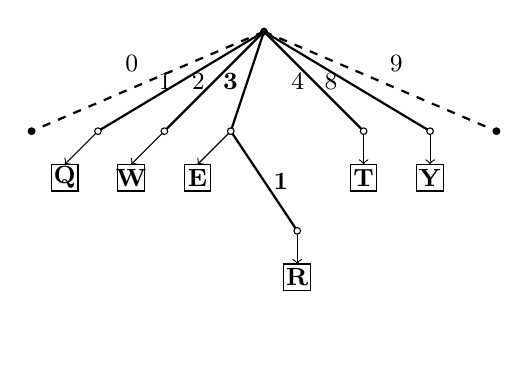
\begin{tikzpicture}[scale=1.2]

\newcommand\Y{-30};
\newcommand\ADDY{-10};

  %% node to node
  \small
  \draw[dashed,thick] (0pt,0pt) -- node[anchor=south east]{0} (-70pt,-30pt);
  \draw[thick] (0pt,0pt) -- node[anchor=east]{1} (-50pt,-30pt); %% Q
  \draw[thick] (0pt,0pt) -- node[anchor=east]{2} (-30pt,-30pt); %% W
  \draw[thick] (0pt,0pt) -- node[anchor=east]{\textbf{3}} (-10pt,-30pt); %% E
  \draw[thick] (0pt,0pt) -- node[anchor=east]{4} ( 30pt,-30pt); %% T
  \draw[thick] (0pt,0pt) -- node[anchor=east]{8} ( 50pt,-30pt); %% Y
  \draw[dashed,thick] (0pt,0pt) -- node[anchor=south west]{9} ( 70pt,-30pt);

  \draw[thick] (-10pt,-30pt) -- node[anchor=west]{\textbf{1}} ( 10pt,-60pt); %% R
%  \draw[thick] (-10pt,-30pt) -- node[anchor=west]{\textbf{0}} (-10pt,-60pt);
%  \draw[thick] (-10pt,-60pt) -- node[anchor=east]{\textbf{X}} (  0pt,-90pt); %% ?


  %% node to element
  \draw[->] (-50pt,\Y pt) -- (-60pt, \ADDY +\Y pt);
  \draw[->] (-30pt,\Y pt) -- (-40pt, \ADDY +\Y pt);
  \draw[->] (-10pt,\Y pt) -- (-20pt, \ADDY +\Y pt);
  \draw[->] ( 30pt,\Y pt) -- ( 30pt, \ADDY +\Y pt);
  \draw[->] ( 50pt,\Y pt) -- ( 50pt, \ADDY +\Y pt);

  \draw[->] ( 10pt,2 * \Y pt) -- ( 10pt, \ADDY + 2 * \Y pt);
%  \draw[->] (  0pt,3 * \Y pt) -- (  0pt, \ADDY + 3 * \Y pt);

  %% nodes
  \draw[fill=black] ( 0pt,  0pt) circle (1pt); 
  \draw[fill=black] (-70pt, -30pt) circle (1pt); 
  \draw[fill=white] (-50pt, -30pt) circle (1pt); %% Q
  \draw[fill=white] (-30pt, -30pt) circle (1pt); %% W
  \draw[fill=white] (-10pt, -30pt) circle (1pt); %% E
  \draw[fill=white] ( 30pt, -30pt) circle (1pt); %% T
  \draw[fill=white] ( 50pt, -30pt) circle (1pt); %% Y
  \draw[fill=black] ( 70pt, -30pt) circle (1pt);

%  \draw[fill=white] (-10pt, 2 * \Y pt) circle (1pt); %% R
  \draw[fill=white] ( 10pt, 2 * \Y pt) circle (1pt); %% x
%  \draw[fill=white] (  0pt, 3 * \Y pt) circle (1pt); %% ?

  %% elements
  \draw[fill=white](-60pt,-4 + \ADDY + \Y pt)
  node{\textbf{Q}} +(-4pt,-4pt) rectangle +(4pt,4pt) ; %% Q
  \draw[fill=white](-40pt,-4 + \ADDY + \Y pt)
  node{\textbf{W}} +(-4pt,-4pt) rectangle +(4pt,4pt) ; %% W
  \draw[fill=white](-20pt,-4 + \ADDY + \Y pt)
  node{\textbf{E}} +(-4pt,-4pt) rectangle +(4pt,4pt) ; %% E
  \draw[fill=white]( 30pt,-4 + \ADDY + \Y pt)
  node{\textbf{T}} +(-4pt,-4pt) rectangle +(4pt,4pt) ; %% T
  \draw[fill=white]( 50pt,-4 + \ADDY + \Y pt)
  node{\textbf{Y}} +(-4pt,-4pt) rectangle +(4pt,4pt) ; %% Y

  \draw[fill=white]( 10pt,-4 + \ADDY + 2 * \Y pt)
  node{\textbf{R}} +(-4pt,-4pt) rectangle +(4pt,4pt) ; %% R
%  \draw[fill=white](  0pt,-4 + \ADDY + 3 * \Y pt)
%  node{\textbf{?}} +(-4pt,-4pt) rectangle +(4pt,4pt) ; %% ?
  \draw(0, -8+\ADDY+ 2.5*\Y pt);

\end{tikzpicture}

%   \caption{\label{fig:treemodelexample} Underlying 10-ary tree $\mathcal{T}$ of
%     a sequence. The paths $\mathcal{P}$ correspond to the concatenation of the
%     edges from the root to the elements. The elements are characters. Using the
%     total order ($\mathcal{P},\, <_\mathcal{P}$), the sequence of elements is
%     $QWERTY$.}
% \end{figure}

% Figure~\ref{fig:treemodelexample} shows the underlying 10-ary tree
% $\mathcal{T}$ representing a sequences. Like in the previous scenario, the
% initial sequence is $QWTY$ with the respective paths $[1]$, $[2]$, $[4]$ and
% $[8]$. The insertion of the character $E$ between the pairs
% $\langle [2],\, W\rangle$ and $\langle [4],\, T\rangle$ results in the
% following pair: $\langle [3],\, E \rangle$. Then the insertion of the character
% $R$ needs to start a new level since there is no room at the first level of the
% tree for a new path between $E$ and $T$. The resulting path may be $[3.1]$ if
% label one is chosen for the element $R$ at the second level. This would
% increase the depth of the tree in case there is an insertion between the
% elements $E$ and $R$. The new path would be $[3.0.X]$ where $0<X<10$ (recall
% that we assumed a 10-ary tree). The total order $(\mathcal{P},\,<_\mathcal{P})$
% allows retrieving the sequence $QWERTY$.

% %% \subsection{Disambiguation of concurrent cases}

% Two collaborators concurrently performing an operation on their respective
% replica may get different results after the integration of both
% operations. Indeed, $(\mathcal{P},\,<_\mathcal{P})$ is a total order when a
% single collaborator edits. However, it becomes a partial order when the editing
% involves several collaborators. Consequently, it is necessary to totally order
% the elements inserted by different collaborators. To this end, the
% disambiguation function $\delta$ associates a disambiguator to each pair of
% $\mathcal{T}$. $\delta: \mathcal{P}\times\mathcal{A} \rightarrow \mathcal{D}$
% such that ($\mathcal{D}$, $<_{\mathcal{D}}$) is a total order. The function
% $\delta$ is an accessor to additional values that are totally ordered even in
% presence of concurrency. Finally, the pairs in $\mathcal{T}$ can be totally
% ordered with a composition of the local total order ($\mathcal{P}$,
% $<_{\mathcal{P}}$) and the total order between collaborators ($\mathcal{D}$,
% $<_{\mathcal{D}}$). The composition leads to a total order ($\mathcal{T}$,
% $<_{\mathcal{T}}$).

% Figure~\ref{fig:desexample} depicts a tree containing 6 elements with only 5
% distinct paths (two values are associated with the path $[3]$). Similarly to
% the previous example, the initial sequence was $QWTY$, however, in this
% example, the two elements $E$ and $R$ are inserted between the pairs
% $\langle [2],\, W\rangle$ and $\langle [4],\,T\rangle$ by two different
% collaborators concurrently. For both elements, the resulting path is
% $[3]$. After the two elements are inserted, the sequence becomes either
% $QWERTY$ or $QWRETY$. Nevertheless, let
% $\delta(\langle [3],\, R \rangle) = \delta_R$ and
% $\delta(\langle [3],\, T\rangle) = \delta_T$. If we assume
% $\delta_R <_\mathcal{D} \delta_T$, the total order
% $(\mathcal{T}, <_\mathcal{T})$ gives the sequence $QWERTY$. It is worth noting
% that disambiguators are usually computed using a monotonically increasing
% variable and a unique collaborator identifier just like Lamport
% timestamps~\cite{lamport1978time}. Therefore, a collaborator cannot directly
% influence the final position of the character in the sequence using
% disambiguators. The sequence of the example could have ended in $QWRETY$ and it
% would have needed a correction.

% \begin{figure}
%   \centering
%   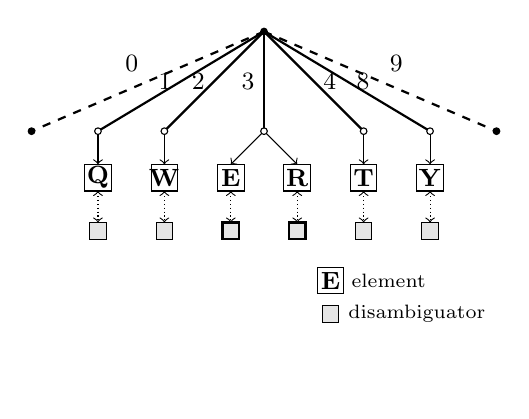
\begin{tikzpicture}[scale=1.2]

\newcommand\Y{-30};
\newcommand\ADDY{-10};

  %% node to node
  \small
  \draw[dashed,thick] (0pt,0pt) -- node[anchor=south east]{0} (-70pt,\Y pt);
  \draw[thick] (0pt,0pt) -- node[anchor=east]{1} (-50pt, \Y pt); %% Q
  \draw[thick] (0pt,0pt) -- node[anchor=east]{2} (-30pt, \Y pt); %% W
  \draw[thick] (0pt,0pt) -- node[anchor=east]{3} (  0pt, \Y pt); %% E R
  \draw[thick] (0pt,0pt) -- node[anchor=west]{4} ( 30pt, \Y pt); %% T
  \draw[thick] (0pt,0pt) -- node[anchor=west]{8} ( 50pt, \Y pt); %% Y
  \draw[dashed,thick] (0pt,0pt) -- node[anchor=south west]{9} ( 70pt, \Y pt);

  %% node to element
  \draw[->] (-50pt,\Y pt) -- (-50pt, \ADDY +\Y pt);
  \draw[->] (-30pt,\Y pt) -- (-30pt, \ADDY +\Y pt);
  \draw[->] (  0pt,\Y pt) -- (-10pt, \ADDY +\Y pt);
  \draw[->] (  0pt,\Y pt) -- ( 10pt, \ADDY +\Y pt);
  \draw[->] ( 30pt,\Y pt) -- ( 30pt, \ADDY +\Y pt);
  \draw[->] ( 50pt,\Y pt) -- ( 50pt, \ADDY +\Y pt);

  %% element to desambiguator
  \draw[<->,densely dotted](-50pt,-8+\ADDY + \Y pt)--(-50pt,2.75*\ADDY+\Y pt);
  \draw[<->,densely dotted](-30pt,-8+\ADDY + \Y pt)--(-30pt,2.75*\ADDY+\Y pt);
  \draw[<->,densely dotted](-10pt,-8+\ADDY + \Y pt)--(-10pt,2.75*\ADDY+\Y pt);
  \draw[<->,densely dotted]( 10pt,-8+\ADDY + \Y pt)--( 10pt,2.75*\ADDY+\Y pt);
  \draw[<->,densely dotted]( 30pt,-8+\ADDY + \Y pt)--( 30pt,2.75*\ADDY+\Y pt);
  \draw[<->,densely dotted]( 50pt,-8+\ADDY + \Y pt)--( 50pt,2.75*\ADDY+\Y pt);

  %% nodes
  \draw[fill=black] ( 0pt, 0 pt) circle (1pt); 
  \draw[fill=black] (-70pt, \Y pt) circle (1pt); 
  \draw[fill=white] (-50pt, \Y pt) circle (1pt); %% Q
  \draw[fill=white] (-30pt, \Y pt) circle (1pt); %% W
  \draw[fill=white] (  0pt, \Y pt) circle (1pt); %% E
  \draw[fill=white] ( 30pt, \Y pt) circle (1pt); %% T
  \draw[fill=white] ( 50pt, \Y pt) circle (1pt); %% Y
  \draw[fill=black] ( 70pt, \Y pt) circle (1pt);

  %% desambiguator
  \draw[fill=gray!20] (-50pt,-2.5+2.75*\ADDY+\Y pt)
  +(-2.5pt,-2.5pt) rectangle +(2.5pt,2.5pt);
  \draw[fill=gray!20] (-30pt,-2.5+2.75*\ADDY+\Y pt)
  +(-2.5pt,-2.5pt) rectangle +(2.5pt,2.5pt);
  \draw[fill=gray!20, thick] (-10pt,-2.5+2.75*\ADDY+\Y pt)
  +(-2.5pt,-2.5pt) rectangle +(2.5pt,2.5pt);
  \draw[fill=gray!20, thick] ( 10pt,-2.5+2.75*\ADDY+\Y pt)
  +(-2.5pt,-2.5pt) rectangle +(2.5pt,2.5pt);
  \draw[fill=gray!20] ( 30pt,-2.5+2.75*\ADDY+\Y pt)
  +(-2.5pt,-2.5pt) rectangle +(2.5pt,2.5pt);
  \draw[fill=gray!20] ( 50pt,-2.5+2.75*\ADDY+\Y pt)
  +(-2.5pt,-2.5pt) rectangle +(2.5pt,2.5pt);

  %% elements
  \draw[fill=white](-50pt,-4 + \ADDY + \Y pt)
  node{\textbf{Q}} +(-4pt,-4pt) rectangle +(4pt,4pt) ; %% Q
  \draw[fill=white](-30pt,-4 + \ADDY + \Y pt)
  node{\textbf{W}} +(-4pt,-4pt) rectangle +(4pt,4pt) ; %% W
  \draw[fill=white](- 10pt,-4 + \ADDY + \Y pt)
  node{\textbf{E}} +(-4pt,-4pt) rectangle +(4pt,4pt) ; %% E
  \draw[fill=white]( 10pt,-4 + \ADDY + \Y pt)
  node{\textbf{R}} +(-4pt,-4pt) rectangle +(4pt,4pt) ; %% R
  \draw[fill=white]( 30pt,-4 + \ADDY + \Y pt)
  node{\textbf{T}} +(-4pt,-4pt) rectangle +(4pt,4pt) ; %% T
  \draw[fill=white]( 50pt,-4 + \ADDY + \Y pt)
  node{\textbf{Y}} +(-4pt,-4pt) rectangle +(4pt,4pt) ; %% Y

  
  \begin{scope}[shift={(20pt, 2.5*\Y pt)}]    
    \draw[fill=white](0,0)node{\textbf{E}} +(-4pt, -4pt) rectangle +(4pt, 4pt);
    \scriptsize
    \draw (4pt, 0)node[anchor=west]{element};
    \draw[fill=gray!20] (0,\ADDY pt) +(-2.5pt, -2.5pt)rectangle+(2.5pt, 2.5pt);
    \draw (3pt, \ADDY pt) node[anchor=west]{disambiguator};
  \end{scope}
  %% spacing
  \draw(0, -8+\ADDY+ 3*\Y pt);

\end{tikzpicture}

%   \caption{\label{fig:desexample}The 10-ary tree of a sequence including
%     concurrent insertions. Using only ($\mathcal{P},\, <_\mathcal{P}$) could
%     lead to either $QWERTY$ or $QWRETY$. The disambiguators forces the final
%     result to converge to $QWERTY$.}
% \end{figure}

% %% \subsection{Choosing the rightful path}
% \label{sec:choosing}

The most critical part of such sequences consists in creating the
paths. Algorithm~\ref{algo:crdtabstract} shows the general outlines of these
sequences. It divides the operations into two different parts, the local and the
remote phases of the optimistic replication paradigm. As we can see, the local
part of the insert operation concentrates most of the complexity where the
algorithm has to generate the identifier composed of the path, i.e., the list of
integers (cf. Line~\ref{line:allocpath}) and a disambiguator to ensure a global
total order (cf. Line~\ref{line:allocdes}).

\begin{algorithm}
  
\small
\algrenewcommand{\algorithmiccomment}[1]{\hskip2em$\rhd$ #1}

\newcommand{\comment}[1]{$\rhd$ #1}


\algblockdefx[initially]{initially}{endInitially}
  [0] {\textbf{INITIALLY:}} 

\algblockdefx[local]{local}{endLocal}
  [0] {\textbf{LOCAL UPDATE:}}

\algblockdefx[received]{received}{endReceived}
  [0] {\textbf{RECEIVED UPDATE:}}

\algblockdefx[onInsert]{onLocal}{endOnLocal}
  [0] {\textbf{on} insert ($p \in \mathcal{I},\,\alpha \in \mathcal{A},\,
   q\in\mathcal{I}$):}
  [0] {\textbf{on} delete ($i \in \mathcal{I}$):} 

\algblockdefx[onRemote]{onRemote}{endOnRemote}
  [0] {\textbf{on} insert ($i\in\mathcal{I}$):\hfill\comment{once per 
  distinct triple in $\mathcal{I}$}}
  [0] {\textbf{on} delete ($i\in\mathcal{I}$):\hfill\comment{after the 
  remote $insert(i)$ is done}} 

\newcommand{\LINEFOR}[2]{%
  \algorithmicfor\ {#1}\ \algorithmicdo\ {#2} %
  }

\newcommand{\LINEIFTHEN}[2]{%
  \algorithmicif\ {#1}\ \algorithmicthen\ {#2} %
  }

\newcommand{\INDSTATE}[1][1]{\State\hspace{\algorithmicindent}}

\begin{algorithmic}[1]
  \Statex
  \initially
    \State $\mathcal{T} \leftarrow \varnothing$; \hfill \comment{structure of
     the CRDT for sequences}
  \endInitially
  
  \local
    \onLocal
    \State \textbf{let} $path \leftarrow allocPath(p.P,\,q.P)$; \label{line:allocpath}
    \State \textbf{let} $dis \leftarrow allocDis(p,\, path,\, q)$; \label{line:allocdes}
    \State $broadcast('insert',\, \langle path,\, \alpha,\, dis \rangle)$;
    \endOnLocal
    \INDSTATE $broadcast('delete',\,i)$;
  \endLocal
  
  \received
    \onRemote
    \State $\mathcal{T} \leftarrow \mathcal{T} \cup i$;
    \endOnRemote
    \INDSTATE $\mathcal{T} \leftarrow \mathcal{T}\, \backslash\, i$; 
  \endReceived
  
\end{algorithmic}

  \caption{\label{algo:crdtabstract}General outlines of a sequence with
    variable-size identifiers.}
\end{algorithm}

\TODO{Let $\mathcal{I}$ be the set of unique triples
$\mathcal{I}: \mathcal{P}\times\mathcal{A}\times\mathcal{D}$. The set of the
elements of a sequence is a subset of $\mathcal{I}$. For any element $i$ of a
sequence ($i \in \mathcal{I}$), let $i.P$, $i.A$, $i.D$ be the respective
accessors to the path, the element, and the disambiguator of element $i$. The
function $allocPath$ chooses a path in the tree between two other paths $p.P$
and $q.P$ where $p<_{\mathcal{T}}q$. This means that element $i$ has to be
inserted between two elements $p$ and $q$ such that $p$ precedes $q$ in the
sequence. However, since it is always create new levels in the tree and thus
new sub-trees, the number of possible paths is infinite, and so is the number
of $allocPath$ functions. Nevertheless, the function $allocPath$ should choose
among the all the possible paths the one having the smallest length in order to
have smaller identifiers keeping good performance. This observation reduces
considerably the number of possible $allocPath$ functions. Still, the
allocation of paths without an \emph{a priori} knowledge of the final sequence
is a non-trivial problem (\ref{sec:problem} depicts the problem abstracted from
the collaborative editing context).}

% \begin{figure}
%   \centering
%   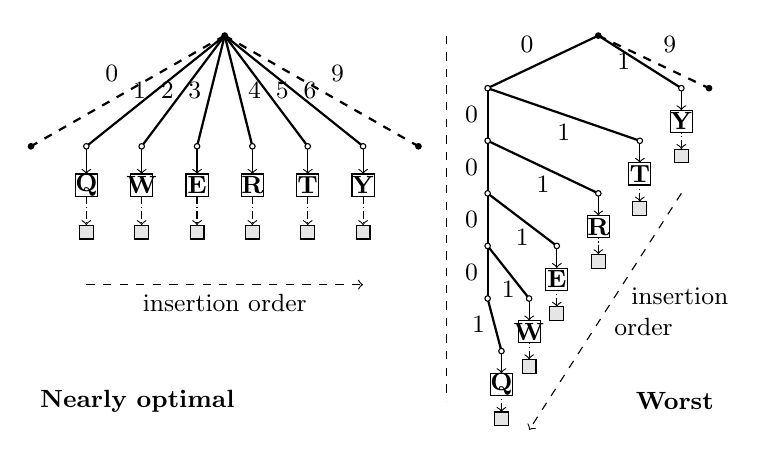
\begin{tikzpicture}[scale=1]

  %% node to node
  \small
  \draw[dashed, thick] (0pt,0pt) -- node[anchor=south east]{0} (-70pt,-40pt);
  \draw[thick] (0pt,0pt) -- node[anchor=east]{1} (-50pt,-40pt);
  \draw[thick] (0pt,0pt) -- node[anchor=east]{2} (-30pt,-40pt);
  \draw[thick] (0pt,0pt) -- node[anchor=east]{3} (-10pt,-40pt);
  \draw[thick] (0pt,0pt) -- node[anchor=west]{4} ( 10pt,-40pt);
  \draw[thick] (0pt,0pt) -- node[anchor=west]{5} ( 30pt,-40pt);
  \draw[thick] (0pt,0pt) -- node[anchor=west]{6} ( 50pt,-40pt);
  \draw[dashed, thick] (0pt,0pt) -- node[anchor=south west]{9} ( 70pt,-40pt);

  %% node to element
  \draw[->] (-50pt,-40pt) -- (-50pt,-50pt);
  \draw[->] (-30pt,-40pt) -- (-30pt,-50pt);
  \draw[->] (-10pt,-40pt) -- (-10pt,-50pt);
  \draw[->] ( 10pt,-40pt) -- ( 10pt,-50pt);
  \draw[->] ( 30pt,-40pt) -- ( 30pt,-50pt);
  \draw[->] ( 50pt,-40pt) -- ( 50pt,-50pt);

  %% element to desambiguator
  \draw[->,densely dashdotted] ( -50pt,-58pt) -- ( -50pt,-68.5pt);
  \draw[->,densely dashdotted] ( -30pt,-58pt) -- ( -30pt,-68.5pt);
  \draw[->,densely dashdotted] ( -10pt,-58pt) -- ( -10pt,-68.5pt);
  \draw[->,densely dashdotted] (  10pt,-58pt) -- (  10pt,-68.5pt);
  \draw[->,densely dashdotted] (  30pt,-58pt) -- (  30pt,-68.5pt);
  \draw[->,densely dashdotted] (  50pt,-58pt) -- (  50pt,-68.5pt);

  \draw[fill=black] (  0pt,  0pt) circle (1pt);
  \draw[fill=black] (-70pt,-40pt) circle (1pt);
  \draw[fill=white] (-50pt,-40pt) circle (1pt);
  \draw[fill=white] (-30pt,-40pt) circle (1pt);
  \draw[fill=white] (-10pt,-40pt) circle (1pt);
  \draw[fill=white] ( 10pt,-40pt) circle (1pt);
  \draw[fill=white] ( 30pt,-40pt) circle (1pt);
  \draw[fill=white] ( 50pt,-40pt) circle (1pt);
  \draw[fill=black] ( 70pt,-40pt) circle (1pt);

  %% elements
  \draw[fill=white](-50pt,-54pt)
  node{\textbf{Q}}+(-4pt,-4pt)rectangle+(4pt,4pt) ;
  \draw[fill=white](50pt,-54pt)
  node{\textbf{Y}} +(-4pt,-4pt) rectangle +(4pt,4pt) ;
  \draw[fill=white]( 10pt,-54pt)
  node{\textbf{R}} +(-4pt,-4pt) rectangle +(4pt,4pt) ;
  \draw[fill=white] ( -30pt,-54pt)
  node{\textbf{W}} +(-4pt,-4pt) rectangle +(4pt,4pt) ;
  \draw[fill=white] ( -10pt,-54pt)
  node{\textbf{E}} +(-4pt,-4pt) rectangle +(4pt,4pt) ;
  \draw[fill=white]( 30pt,-54pt)
  node{\textbf{T}} +(-4pt,-4pt) rectangle +(4pt,4pt) ;

  %% desambiguator
  \draw[fill=gray!20] (-50pt,-71pt) +(-2.5pt,-2.5pt) rectangle +(2.5pt,2.5pt);
  \draw[fill=gray!20] (-30pt,-71pt) +(-2.5pt,-2.5pt) rectangle +(2.5pt,2.5pt);
  \draw[fill=gray!20] (-10pt,-71pt) +(-2.5pt,-2.5pt) rectangle +(2.5pt,2.5pt);
  \draw[fill=gray!20] ( 10pt,-71pt) +(-2.5pt,-2.5pt) rectangle +(2.5pt,2.5pt);
  \draw[fill=gray!20] ( 30pt,-71pt) +(-2.5pt,-2.5pt) rectangle +(2.5pt,2.5pt);
  \draw[fill=gray!20] ( 50pt,-71pt) +(-2.5pt,-2.5pt) rectangle +(2.5pt,2.5pt);

  %% insertion order
  \draw[->,dashed] (-50pt, -90pt) -- node[anchor=north]{insertion order}
  (50pt, -90pt);

%%%%%%%%%%%%%%%%%%%%%%%%%%%%%%%%%%%%%%%%%%%%%%%%%%%%%%%%%%%%%%%%%%%%%%

  \draw[dashed] (80pt,0pt) -- (80pt,-132pt);
  
  \draw (-70pt, -132pt)node[anchor=west]{\textbf{Nearly optimal}};


\begin{scope}[shift={(135pt,0pt)}]

\newcommand\Y{-19}
\newcommand\ADDY{-8}

  \draw (45pt, -132pt) node[anchor=east]{\textbf{Worst}};  

  %% node to node
  \small
  \draw[thick] (0pt,0pt) -- node[anchor=south east]{0} (-40pt,\Y pt);
  \draw[thick] (0pt,0pt) -- node[anchor=east]{1} (30pt, \Y pt); %% Y
  \draw[thick] (-40pt, \Y pt) -- node[anchor=north]{1} (15pt, 2 * \Y pt); %% T
  \draw[thick] (-40pt, \Y pt) -- node[anchor=east]{0} (-40pt, 2 * \Y pt); %% 0
  \draw[thick] (-40pt, 2*\Y pt) -- node[anchor=north]{1} (0pt, 3 * \Y pt); %% R
  \draw[thick] (-40pt, 2*\Y pt)-- node[anchor=east]{0}(-40pt, 3 * \Y pt); %% 0
  \draw[thick] (-40pt, 3*\Y pt) -- node[anchor=north]{1}(-15pt,4 * \Y pt); %% E
  \draw[thick] (-40pt, 3*\Y pt) -- node[anchor=east]{0}(-40pt,4 * \Y pt); %% 0
  \draw[thick] (-40pt, 4*\Y pt) -- node[anchor=north]{1}(-25pt,5 * \Y pt); %% W
  \draw[thick] (-40pt, 4*\Y pt) -- node[anchor=east]{0}(-40pt,5 * \Y pt); %% 0
  \draw[thick] (-40pt, 5*\Y pt) -- node[anchor=east]{1}(-35pt,6 * \Y pt); %% Q

  \draw[dashed, thick] (0pt,0pt) -- node[anchor=south west]{9} (40pt,\Y pt);

  %% node to element
  \draw[->] ( 30pt, \Y pt) -- ( 30pt, \ADDY + \Y pt); %% Y
  \draw[->] ( 15pt, 2* \Y pt) -- ( 15pt, \ADDY + 2 *\Y pt); %% T
  \draw[->] (  0pt, 3 *\Y pt) -- (  0pt, \ADDY + 3 *\Y pt); %% R
  \draw[->] (-15pt, 4 *\Y pt) -- ( -15pt, \ADDY + 4 *\Y pt); %% E
  \draw[->] (-25pt, 5 *\Y pt) -- ( -25pt, \ADDY + 5 *\Y pt); %% W
  \draw[->] (-35pt, 6 *\Y pt) -- ( -35pt, \ADDY + 6 *\Y pt); %% Q

  %% element to desambiguator
  \draw[->,densely dashdotted]
  ( 30pt, \ADDY + \Y pt) -- ( 30pt,2.75*\ADDY+\Y pt); %% Y
  \draw[->,densely dashdotted]
  ( 15pt, \ADDY + 2* \Y pt) -- ( 15pt,2.75*\ADDY+ 2* \Y pt); %% T
  \draw[->,densely dashdotted]
  ( 0pt, \ADDY + 3* \Y pt) -- (  0pt,2.75*\ADDY+ 3* \Y pt); %% R
  \draw[->,densely dashdotted]
  ( -15pt, \ADDY + 4 *\Y pt) -- ( -15pt,2.75*\ADDY+ 4* \Y pt); %% E
  \draw[->,densely dashdotted]
  ( -25pt, \ADDY + 5 *\Y pt) -- ( -25pt,2.75*\ADDY+ 5*\Y pt); %% W
  \draw[->,densely dashdotted]
  ( -35pt, \ADDY + 6* \Y pt) -- ( -35pt,2.75*\ADDY+ 6*\Y pt); %% Q

  %% node
  \draw[fill=black] (0pt,0pt) circle (1pt); %% rooot
  \draw[fill=white] ( 30pt, \Y pt) circle (1pt); %% Y
  \draw[fill=white] (-40pt, \Y pt) circle (1pt); %% 0
  \draw[fill=white] ( 15 pt, 2 * \Y pt) circle (1pt); %% T
  \draw[fill=white] (-40pt, 2 * \Y pt) circle (1pt); %% 0
  \draw[fill=white] (  0 pt, 3 * \Y pt) circle (1pt); %% R
  \draw[fill=white] (-40pt, 3 * \Y pt) circle (1pt); %% 0
  \draw[fill=white] (-15 pt, 4 * \Y pt) circle (1pt); %% E
  \draw[fill=white] (-40pt, 4 * \Y pt) circle (1pt); %% 0
  \draw[fill=white] (-25 pt, 5 * \Y pt) circle (1pt); %% W
  \draw[fill=white] (-40pt, 5 * \Y pt) circle (1pt); %% 0
  \draw[fill=white] (-35 pt, 6 * \Y pt) circle (1pt); %% Q

  \draw[fill=black] ( 40pt, \Y pt) circle (1pt);


  %% elements
  \draw[fill=white] ( 30pt, -4 + \ADDY + \Y pt)
  node{\textbf{Y}} +(-4pt,-4pt) rectangle +(4pt,4pt) ; %% Y
  \draw[fill=white] ( 15pt, -4 + \ADDY +  2 *\Y pt)
  node{\textbf{T}} +(-4pt,-4pt) rectangle +(4pt,4pt) ; %% T
  \draw[fill=white] (  0pt, -4 + \ADDY +  3* \Y pt)
  node{\textbf{R}} +(-4pt,-4pt) rectangle +(4pt,4pt) ; %% R
  \draw[fill=white] (-15pt, -4 + \ADDY + 4 *\Y pt)
  node{\textbf{E}} +(-4pt,-4pt) rectangle +(4pt,4pt) ; %% E
  \draw[fill=white] (-25pt, -4 + \ADDY + 5 * \Y pt)
  node{\textbf{W}} +(-4pt,-4pt) rectangle +(4pt,4pt) ; %% W
  \draw[fill=white] (-35pt, -4 + \ADDY + 6 *\Y pt)
  node{\textbf{Q}} +(-4pt,-4pt) rectangle +(4pt,4pt) ; %% Q

  %% desambiguator
  \draw[fill=gray!20]( 30pt, -2.5 + 2.75 * \ADDY + \Y pt)
  +(-2.5pt,-2.5pt) rectangle +(2.5pt,2.5pt);
  \draw[fill=gray!20]( 15pt, -2.5 + 2.75 * \ADDY +2 *\Y pt)
  +(-2.5pt,-2.5pt) rectangle +(2.5pt,2.5pt);
  \draw[fill=gray!20](  0pt, -2.5 + 2.75 * \ADDY + 3*\Y pt)
  +(-2.5pt,-2.5pt) rectangle +(2.5pt,2.5pt);
  \draw[fill=gray!20](-15pt, -2.5 + 2.75 * \ADDY +4*\Y pt )
  +(-2.5pt,-2.5pt) rectangle +(2.5pt,2.5pt);
  \draw[fill=gray!20](-25pt, -2.5 + 2.75 * \ADDY + 5*\Y pt)
  +(-2.5pt,-2.5pt) rectangle +(2.5pt,2.5pt);
  \draw[fill=gray!20](-35pt, -2.5 + 2.75 * \ADDY +6*\Y pt) 
  +(-2.5pt,-2.5pt) rectangle +(2.5pt,2.5pt);

  %% insertion order
  \draw[->,dashed] (30pt, 3 * \Y pt) -- node[anchor=west,align=left]
  {\ \ insertion\\ order} (-25pt, 7.5 * \Y pt);


\end{scope}

\end{tikzpicture}

%   \caption{\label{fig:allocpathexample} Two trees filled with the resulting
%     identifiers of two different permutations resulting in an identical
%     sequence $QWERTY$. They use the same function $allocPath$ which allocates
%     the leftmost branch in the tree. All paths of the nearly optimal case have
%     a length of 1 while the tree of the worst case grows up to a depth of 6.}
% \end{figure}

% Figure~\ref{fig:allocpathexample} illustrates the difficulties of designing a
% function to allocate the paths. It represents the underlying trees of two
% sequences using the allocation function: they allocate the leftmost branch
% available at the lowest depth possible. In both cases the final sequence is
% $QWERTY$, however, the letters are not inserted in the same order. In the first
% case, $Q$ is inserted first at position 0 (initially the sequence is empty),
% followed by $W$ at position 1 (after $Q$) then $E$ is inserted at position 3
% (after $W$), etc. We call the sequence of insert operations $[(Q,\,0)$,
% $(W,\,1)$, $(E,\,2)$, $\ldots]$ the \emph{editing sequence}. In the second
% case, the letter $Y$ is inserted first at position 0 as the sequence is
% initially empty. Then $T$ is inserted. However as the final intended word is
% $QWERTY$, $T$ has to be inserted at a position before $Y$ that represents the
% current state of the sequence. $T$ is thus inserted at position 0 shifting $Y$
% to position $1$, etc. The editing sequence that corresponds to this case
% is thus $[(Y,\,0)$, $(T,\,0)$, $(R,\,0)$, $\ldots]$.

% \begin{itemize}[leftmargin=*]
% \item Case 1: Since the function $allocPath$ allocates the leftmost branches,
%   the following editing sequence $[(Q,\,0)$, $(W,\,1)$, $(E,\,2)$, $\ldots]$
%   leads to the paths $\langle [1],\, Q\rangle$, $\langle [2],\, W\rangle$,
%   $\langle [3],\, E\rangle$, etc. In this case, the depth of the tree never
%   grows. In this regard, this function $allocPath$ is very efficient in terms
%   of the size of the allocated identifiers.

% \item Case 2: The editing sequence $[(Y,\,0)$, $(T,\,0)$, $(R,\,0)$, $\ldots]$
%   leads to an increase of the depth of the tree at each element
%   insertion. Indeed, as an element gets the smallest value at its level
%   (cf. the allocation function), there is no way to insert a new element before
%   at the same level hence the new level. The resulting sequence is
%   $\langle [1],\, Y\rangle$, $\langle [0.1],\, T\rangle$,
%   $\langle [0.0.1],\, R \rangle$, etc. Consequently, the size of the paths
%   grows very fast.
% \end{itemize}

% This example shows how the insertion order impacts the length of the allocated
% paths. Unfortunately, the insertion order cannot be predicted, nor the size of
% the final sequence. Prior work on sequences often made the assumption of a
% left-to-right editing due to observations made on
% corpus~\cite{preguica2009commutative, weiss2009logoot}. However, there exist
% human edited documents that do not correspond to this kind of
% editing~\cite{nedelec2013lseq}. Indeed, the editing depends on the type of the
% document and to the activity for example when correcting a document the editing
% in mainly random as the insertions/deletions may correspond to
% errors. Consequently, we are looking for an allocation function which provides
% identifiers with a sub-linear spatial complexity compared to the number of
% insertions whatever is the editing sequence.

\subsection{Scalable information dissemination}

To provide the eventual consistency of the aforementioned optimistic
replication approach, the application must disseminate the result of operations
to all participants of the editing session, i.e., broadcast the
operations. Since the number of these participants is possibly large,
participants cannot afford the full knowledge of the membership. Instead, the
common scalable approach consists in keeping a small list of known members
(referred as \emph{neighbors}) and send them operations. Then, each neighbors
forwards the operations to their own neighborhood. Thus, from
neighbors-to-neighbors, the operations reach all members.

The recent WebRTC technology allows establishing peer-to-peer connections inside
web browsers. As such, it allows creating an overlay network between web
browsers. Nevertheless, WebRTC imposes a complex and costly connection protocol.
Indeed, as depicted in \TODO{Figure}, a user $u_1$ wishing to establish a
connection with a user $u_2$ must create an offer ticket and send it to $u_2$
through a mediator (e.g. by mail, dedicated servers, peers already connected in
the network). Then, $u_2$ must answer with another offer (refereed as
\emph{stamped ticket}) using a mediator too. Finally, $u_1$ must confirm the
connection to establish the bidirectional link.

%%% Local Variables: 
%%% mode: latex
%%% TeX-master: "../paper"
%%% End: 


\newcommand{\PARAGRAPH}{-20pt}
\newcommand{\ABOVETABLES}{8pt}

\section{LSeq: a polylogarithmic path \nohyphens{allocator}}
\label{sec:proposal}

\LSEQ (poly\textsc{L}ogarithmic \textsc{SEQ}uence) is the name of the proposed
allocation function.
Our prior works~\cite{nedelec2013concurrency, nedelec2013lseq} empirically
showed that \LSEQ allocates identifiers with a sublinear upper bound on space
complexity.  However, we did not provide any complexity analysis to support
these observations.

This section starts by describing the allocation strategy. Then, it provides the
proof of the polylogarithmic growth of \LSEQ's identifiers and states the
conditions upon which this applies. The complexity analysis also includes the
space complexity of a replicated structure, and the time complexity of
operations provided by such structure.

\noindent As for the communication complexity, the next section describes
an \LSEQ-based editor that benefits from these identifiers.

\subsection{Allocation of paths}
\label{subsec:lseqallocation}

When a user types a character, the editor executes the local part of the
\textsc{insert} operation (see Line~\ref{line:insert} of
Algorithm~\ref{algo:crdtabstract}). This function allocates an identifier
comprising a path, the element, and a disambiguator. The most important choice
concerns the path (see Line~\ref{line:allocpath} of
Algorithm~\ref{algo:crdtabstract}).
\noindent The function \textsc{allocPath} chooses the path that encodes the
position of the new element regarding its adjacent elements in the sequence
using a dense space. For the sake of performance, it aims to keep the paths
small.

\begin{algorithm}

\begin{algorithm}[h]
\small
\algrenewcommand{\algorithmiccomment}[1]{\hskip2em$\rhd$ #1}
\newcommand*{\comment}[1]{$\rhd$ #1}

  \begin{algorithmic}[1]
  \State \textbf{let} $boundary \leftarrow 10$; \Comment{Any constant} 
  \State \textbf{let} $h:\mathbb{N} \rightarrow (\mathcal{P}\times
  \mathcal{P}\rightarrow \mathcal{P})$; \hfill \comment{get sub-allocation
    function}
  \Statex
    \Function{allocPath}{$p,\, q \in \mathcal{P}$}
    $\rightarrow \mathcal{P}$
    \State \textbf{let} $depth,\,\_ \leftarrow getDepthInterval(p,\,q)$;
    \State \textbf{return} $h(depth)(p,\,q)$; \Comment{Defers the call}
    \EndFunction
    \Statex
    \Function{endEditing}{$p,\,q \in \mathcal{P}$}
    $\rightarrow \mathcal{P}$
    \Statex \comment{\#1 Get the depth of the new path}
    \State \textbf{let} $depth,\,interval \leftarrow getDepthInterval(p,q);$
    \Statex \comment{\#2 Process a maximal space between two identifiers}
    \State \textbf{let} $step \leftarrow min(boundary,interval)$;
    \Statex \comment{\#3 Create the new path}
    \State \textbf{return} $subPath(p,depth) + rand(0,step)$;
    \EndFunction
    \Statex
    \Function{frontEditing}{$p,\,q \in \mathcal{P}$}
    $\rightarrow \mathcal{P}$
    \State \textbf{let} $depth,\, interval \leftarrow getDepthInterval(p,q);$
    \hfill \comment{\#1}
    \State \textbf{let} $step \leftarrow min(boundary,interval)$;
    \hfill \comment{\#2}
    \State \textbf{return} $subPath(q,depth) - rand(0,step)$;
    \hfill \comment{\#3}
    \EndFunction

    \Statex 
    \Statex 
    \comment{Which depth has enough space for 1 path}
    \Function{getDepthInterval}{$p,\,q \in \mathcal{P}$} $\rightarrow \mathbb{N} \times \mathbb{N}$
      \State \textbf{let} $depth \leftarrow 0$; $interval \leftarrow 0$;
      \While{$(interval < 2)$}
        \State $depth \leftarrow depth + 1$;
        \State $interval \leftarrow subPath(q,depth) - subPath(p,depth)$;
      \EndWhile
      \State \textbf{return} $\langle depth,\, interval\rangle$;
    \EndFunction

  \end{algorithmic}
\caption{The $allocPath$ function of \NAME{}}
\label{algo:allocpathalgo}

\end{algorithm}

\caption{\label{algo:allocpath}Allocation of paths}
\end{algorithm}

Algorithm~\ref{algo:allocpath} shows the instructions of \LSEQ that implements
\textsc{allocPath}, and Figure~\ref{fig:lseqtreeexample} shows the tree filled
with the identifiers generated by this algorithm on the scenarios presented in
Figure~\ref{fig:allocpathexample}. Figure~\ref{fig:lseqtreeexampleA} describes
the left-to-right insertions of characters resulting in \texttt{QWERTY}
i.e. [($\texttt{Q},\,0$), ($\texttt{W},\,1$),
\ldots]. Figure~\ref{fig:lseqtreeexampleB} describes the right-to-left
insertions of characters resulting in \texttt{QWERTY} i.e.  [($\texttt{Y},\,0$),
($\texttt{T},\,0$), \ldots].

\begin{figure*}
  \centering
  \subfloat[Left-to-right case with \LSEQ.]
  [\label{fig:lseqtreeexampleA} Left-to-right editing behavior.]
  {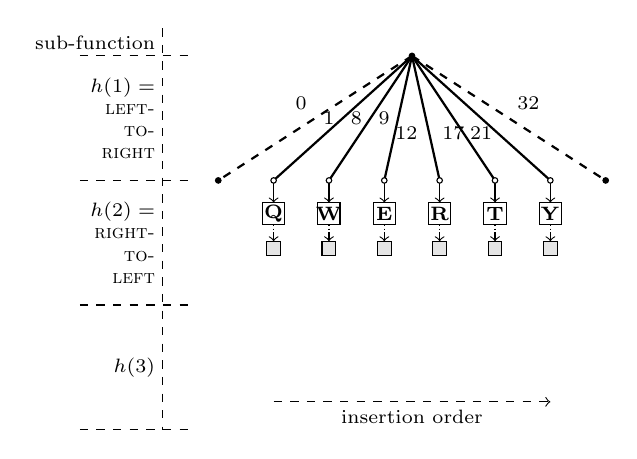
\begin{tikzpicture}[scale=1.]

\newcommand\Y{-45}
\newcommand\ADDY{-8}

  \scriptsize
  \draw[dashed] (0pt,10pt) node[anchor=north east]{sub-function} -- (0pt,3*\Y pt);
  \draw[dashed] (-30pt,0 pt) -- (10pt,0 pt);
  \draw[dashed] (-30pt,\Y pt) -- (10pt,\Y pt);
  \draw[dashed] (-30pt,2*\Y pt) -- (10pt,2*\Y pt);
  \draw[dashed] (-30pt,3*\Y pt) -- (10pt,3*\Y pt);

  \draw (0pt,0.5*\Y pt)
  node[anchor=east, align=right]{$h(1) =$\\\textsc{left-}\\\textsc{to-}\\\textsc{right}};
  \draw (0pt,1.5*\Y pt)
  node[anchor=east, align=right]{$h(2) =$\\\textsc{right-}\\\textsc{to-}\\\textsc{left}};
  \draw (0pt,2.5*\Y pt)
  node[anchor=east]{$h(3)$};

  \begin{scope}[shift={(90pt,0pt)}]
  \draw[->,dashed](-50pt,3*\Y + 10 pt) -- node[anchor=north]{insertion order}
  (50pt, 3*\Y + 10 pt);

  %% node to node
  \scriptsize
  \draw[dashed, thick] (0pt,0pt) -- node[anchor=south east]{0} (-70pt,\Y pt);
  \draw[thick] (0pt,0pt) -- node[anchor=east]{1} (-50pt,\Y pt);
  \draw[thick] (0pt,0pt) -- node[anchor=east]{8} (-30pt,\Y pt);
  \draw[thick] (0pt,0pt) -- node[anchor=east]{9} (-10pt,\Y pt);
  \draw[thick] (0pt,0pt) -- node[anchor=north east]{12} ( 10pt,\Y pt);
  \draw[thick] (0pt,0pt) -- node[anchor=north]{17} ( 30pt,\Y pt);
  \draw[thick] (0pt,0pt) -- node[anchor=north]{21} ( 50pt,\Y pt);
  \draw[dashed, thick] (0pt,0pt) -- node[anchor=south west]{32} ( 70pt,\Y pt);
  %% node to element
  \draw[->] (-50pt,\Y pt) -- (-50pt,\ADDY + \Y pt);
  \draw[->] (-30pt,\Y pt) -- (-30pt,\ADDY + \Y pt);
  \draw[->] (-10pt,\Y pt) -- (-10pt,\ADDY + \Y pt);
  \draw[->] ( 10pt,\Y pt) -- ( 10pt,\ADDY + \Y pt);
  \draw[->] ( 30pt,\Y pt) -- ( 30pt,\ADDY + \Y pt);
  \draw[->] ( 50pt,\Y pt) -- ( 50pt,\ADDY + \Y pt);

  %% element to desambiguator
  \draw[->,densely dashdotted] ( -50pt,\ADDY + \Y pt) --
  ( -50pt,2.75*\ADDY + \Y pt);
  \draw[->,densely dashdotted] ( -30pt,\ADDY + \Y pt) --
  ( -30pt,2.75*\ADDY + \Y pt);
  \draw[->,densely dashdotted] ( -10pt,\ADDY + \Y pt) --
  ( -10pt,2.75*\ADDY + \Y pt);
  \draw[->,densely dashdotted] (  10pt,\ADDY + \Y pt) --
  (  10pt,2.75*\ADDY + \Y pt);
  \draw[->,densely dashdotted] (  30pt,\ADDY + \Y pt) --
  (  30pt,2.75*\ADDY + \Y pt);
  \draw[->,densely dashdotted] (  50pt,\ADDY + \Y pt) --
  (  50pt,2.75*\ADDY + \Y pt);

  \draw[fill=black] (  0pt,  0pt) circle (1pt);
  \draw[fill=black] (-70pt,\Y pt) circle (1pt);
  \draw[fill=white] (-50pt,\Y pt) circle (1pt);
  \draw[fill=white] (-30pt,\Y pt) circle (1pt);
  \draw[fill=white] (-10pt,\Y pt) circle (1pt);
  \draw[fill=white] ( 10pt,\Y pt) circle (1pt);
  \draw[fill=white] ( 30pt,\Y pt) circle (1pt);
  \draw[fill=white] ( 50pt,\Y pt) circle (1pt);
  \draw[fill=black] ( 70pt,\Y pt) circle (1pt);

  %% elements
  \draw[fill=white](-50pt,-4 + \ADDY + \Y pt)
  node{\textbf{Q}}+(-4pt,-4pt)rectangle+(4pt,4pt) ;
  \draw[fill=white](50pt,-4 + \ADDY + \Y pt)
  node{\textbf{Y}} +(-4pt,-4pt) rectangle +(4pt,4pt) ;
  \draw[fill=white]( 10pt,-4 + \ADDY + \Y pt)
  node{\textbf{R}} +(-4pt,-4pt) rectangle +(4pt,4pt) ;
  \draw[fill=white] ( -30pt,-4 + \ADDY + \Y pt)
  node{\textbf{W}} +(-4pt,-4pt) rectangle +(4pt,4pt) ;
  \draw[fill=white] ( -10pt,-4 + \ADDY + \Y pt)
  node{\textbf{E}} +(-4pt,-4pt) rectangle +(4pt,4pt) ;
  \draw[fill=white]( 30pt,-4 + \ADDY + \Y pt)
  node{\textbf{T}} +(-4pt,-4pt) rectangle +(4pt,4pt) ;

  %% desambiguator
  \draw[fill=gray!20] (-50pt,-2.5 + 2.75 * \ADDY + \Y pt)
  +(-2.5pt,-2.5pt) rectangle +(2.5pt,2.5pt);
  \draw[fill=gray!20] (-30pt,-2.5 + 2.75 * \ADDY + \Y pt)
  +(-2.5pt,-2.5pt) rectangle +(2.5pt,2.5pt);
  \draw[fill=gray!20] (-10pt,-2.5 + 2.75 * \ADDY + \Y pt)
  +(-2.5pt,-2.5pt) rectangle +(2.5pt,2.5pt);
  \draw[fill=gray!20] ( 10pt,-2.5 + 2.75 * \ADDY + \Y pt)
  +(-2.5pt,-2.5pt) rectangle +(2.5pt,2.5pt);
  \draw[fill=gray!20] ( 30pt,-2.5 + 2.75 * \ADDY + \Y pt)
  +(-2.5pt,-2.5pt) rectangle +(2.5pt,2.5pt);
  \draw[fill=gray!20] ( 50pt,-2.5 + 2.75 * \ADDY + \Y pt)
  +(-2.5pt,-2.5pt) rectangle +(2.5pt,2.5pt);

%%%%%%%%%%%%%%%%%%%%%%%%%%%%%%%%%%%%%%%%%%%%%%%%%%%%%%%%%%%%%%%%%%%%%%

\end{scope}

\end{tikzpicture}
}
  \subfloat[Right-to-left case with \LSEQ.]
  [\label{fig:lseqtreeexampleB} Right-to-left editing behavior.]
  {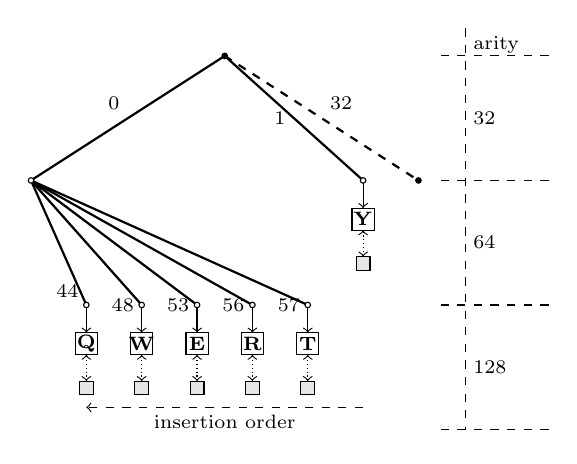
\begin{tikzpicture}[scale=1.]

\newcommand\Y{-45}
\newcommand\ADDY{-10}

  \scriptsize
  \draw[dashed] (340pt,10pt) node[anchor=north west]{arity}  -- (340pt,3*\Y pt);
  \draw[dashed] (370pt,0 pt)  --(330pt,0 pt);
  \draw[dashed] (370pt,\Y pt) -- (330pt,\Y pt);
  \draw[dashed] (370pt,2*\Y pt) -- (330pt,2*\Y pt);
  \draw[dashed] (370pt,3*\Y pt) -- (330pt,3*\Y pt);

  \draw (340pt,0.5*\Y pt)
  node[anchor=west, align=center]{$32$};
  \draw (340pt,1.5*\Y pt)
  node[anchor=west, align=center]{$64$};
  \draw (340pt,2.5*\Y pt)
  node[anchor=west, align=center]{$128$};

  \begin{scope}[shift={(93pt,0pt)}]
    \begin{scope}[shift={(160pt,0pt)}]
  \draw[->,dashed](50pt,3*\Y + 8 pt)--node[anchor=north]{insertion order}
  (-50pt,3*\Y + 8 pt);
  %% node to node
  \scriptsize
  \draw[thick] (0pt,0pt) -- node[anchor=south east]{0} (-70pt,\Y pt);
  \draw[thick] (0pt,0pt) -- node[anchor=east]{1} (50pt, \Y pt); %% Y
  \draw[thick] (-70pt, \Y pt) -- (30pt, 2 * \Y pt); %% T
  \draw[thick] (-70pt, \Y pt) -- (10pt, 2 * \Y pt); %% R
  \draw[thick] (-70pt, \Y pt) -- (-10pt, 2 * \Y pt);%% E
  \draw[thick] (-70pt, \Y pt) -- (-30pt,2 * \Y pt); %% W
  \draw[thick] (-70pt, \Y pt) -- (-50pt,2 * \Y pt); %% Q
  \draw[dashed, thick] (0pt,0pt) -- node[anchor=south west]{32} (70pt,\Y pt);

  %% node to element
  \draw[->] ( 50pt, \Y pt) -- ( 50pt, \ADDY + \Y pt); %% Y
  \draw[->] ( 30pt, 2* \Y pt) -- ( 30pt, \ADDY + 2 *\Y pt); %% T
  \draw[->] ( 10pt, 2 *\Y pt) -- ( 10pt, \ADDY + 2 *\Y pt); %% R
  \draw[->] (-10pt, 2 *\Y pt) -- (-10pt, \ADDY + 2 *\Y pt); %% E
  \draw[->] (-30pt, 2 *\Y pt) -- (-30pt, \ADDY + 2 *\Y pt); %% W
  \draw[->] (-50pt, 2 *\Y pt) -- (-50pt, \ADDY + 2 *\Y pt); %% Q

  %% element to desambiguator
  \draw[<->,densely dotted]
  ( 50pt,-8+ \ADDY + \Y pt) -- ( 50pt,2.75*\ADDY+\Y pt); %% Y
  \draw[<->,densely dotted]
  ( 30pt,-8+ \ADDY + 2* \Y pt) -- ( 30pt,2.75*\ADDY+ 2* \Y pt); %% T
  \draw[<->,densely dotted]
  ( 10pt,-8+ \ADDY + 2* \Y pt) -- ( 10pt,2.75*\ADDY+ 2* \Y pt); %% R
  \draw[<->,densely dotted]
  ( -10pt,-8+ \ADDY + 2 *\Y pt) -- (-10pt,2.75*\ADDY+ 2* \Y pt); %% E
  \draw[<->,densely dotted]
  ( -30pt,-8+ \ADDY + 2 *\Y pt) -- (-30pt,2.75*\ADDY+ 2*\Y pt); %% W
  \draw[<->,densely dotted]
  ( -50pt,-8+ \ADDY + 2* \Y pt) -- (-50pt,2.75*\ADDY+ 2*\Y pt); %% Q

  %% node
  \draw[fill=black] (0pt,0pt) circle (1pt); %% rooot
  \draw[fill=white] ( 50pt, \Y pt) circle (1pt); %% Y
  \draw[fill=white] (-70pt, \Y pt) circle (1pt); %% 0
  \draw[fill=white] ( 30 pt, 2 * \Y pt) node[anchor=east]{57} circle (1pt); %% T
  \draw[fill=white] ( 10 pt, 2 * \Y pt) node[anchor=east]{56} circle (1pt); %% R
  \draw[fill=white] (-10 pt, 2 * \Y pt) node[anchor=east]{53} circle (1pt); %% E
  \draw[fill=white] (-30 pt, 2 * \Y pt) node[anchor=east]{48} circle (1pt); %% W
  \draw[fill=white] (-50 pt, 2 * \Y pt) node[anchor=south east]{44}circle (1pt); %% Q
  \draw[fill=black] ( 70pt, \Y pt) circle (1pt);


  %% elements
  \draw[fill=white] ( 50pt, -4 + \ADDY + \Y pt)
  node{\textbf{Y}} +(-4pt,-4pt) rectangle +(4pt,4pt) ; %% Y
  \draw[fill=white] ( 30pt, -4 + \ADDY +  2 *\Y pt)
  node{\textbf{T}} +(-4pt,-4pt) rectangle +(4pt,4pt) ; %% T
  \draw[fill=white] ( 10pt, -4 + \ADDY +  2* \Y pt)
  node{\textbf{R}} +(-4pt,-4pt) rectangle +(4pt,4pt) ; %% R
  \draw[fill=white] (-10pt, -4 + \ADDY + 2 *\Y pt)
  node{\textbf{E}} +(-4pt,-4pt) rectangle +(4pt,4pt) ; %% E
  \draw[fill=white] (-30pt, -4 + \ADDY + 2 * \Y pt)
  node{\textbf{W}} +(-4pt,-4pt) rectangle +(4pt,4pt) ; %% W
  \draw[fill=white] (-50pt, -4 + \ADDY + 2 *\Y pt)
  node{\textbf{Q}} +(-4pt,-4pt) rectangle +(4pt,4pt) ; %% Q

  %% desambiguator
  \draw[fill=gray!20]( 50pt, -2.5 + 2.75 * \ADDY + \Y pt)
  +(-2.5pt,-2.5pt) rectangle +(2.5pt,2.5pt);
  \draw[fill=gray!20]( 30pt, -2.5 + 2.75 * \ADDY +2 *\Y pt)
  +(-2.5pt,-2.5pt) rectangle +(2.5pt,2.5pt);
  \draw[fill=gray!20]( 10pt, -2.5 + 2.75 * \ADDY +2*\Y pt)
  +(-2.5pt,-2.5pt) rectangle +(2.5pt,2.5pt);
  \draw[fill=gray!20](-10pt, -2.5 + 2.75 * \ADDY +2*\Y pt )
  +(-2.5pt,-2.5pt) rectangle +(2.5pt,2.5pt);
  \draw[fill=gray!20](-30pt, -2.5 + 2.75 * \ADDY +2*\Y pt)
  +(-2.5pt,-2.5pt) rectangle +(2.5pt,2.5pt);
  \draw[fill=gray!20](-50pt, -2.5 + 2.75 * \ADDY +2*\Y pt) 
  +(-2.5pt,-2.5pt) rectangle +(2.5pt,2.5pt);

\end{scope}
\end{scope}

\end{tikzpicture}
}
  \caption{\label{fig:lseqtreeexample} Example of \LSEQ's exponential trees with
    two antagonist editing behaviors to create the sequence of characters
    \texttt{QWERTY}. Contrarily to the example of
    Figure~\ref{fig:allocpathexample}, the depth of trees does not grow
    linearly.}
\end{figure*}

As shown in Figure~\ref{fig:lseqtreeexample}, there exists two major differences
between \LSEQ and the state-of-the-art~\cite{preguica2009commutative,
  weiss2009logoot}:
\begin{itemize}
\item The set of possible paths in \LSEQ can be represented as an exponential
  tree~\cite{andersson1996faster,andersson2007dynamic} instead of a tree of
  constant arity. An exponential tree allows each node to have twice as many
  children as its parent. For instance, in Figure~\ref{fig:lseqtreeexample}, the
  root of the tree can have up to 32 children, each of these children can have
  up to 64 children, etc. This allows to give more space where it is required.
\item Each level of the tree has a different strategy to allocate paths. We can
  see on Figure~\ref{fig:lseqtreeexampleA} that level $h(1)$ allocates paths
  from left to right. The allocated paths increase from 1 to 21. We also see on
  Figure~\ref{fig:lseqtreeexampleB} that level $h(2)$ allocates from right to
  left. The allocated paths decrease from 57 down to 44.
  
\end{itemize}

% General idea.
If the strategy for a level suits the insertion order, then the allocation is
efficient. Otherwise, the level is sacrificed (e.g. the first level in
Figure~\ref{fig:lseqtreeexampleB}) and the next level is efficiently filled.
Thanks to the exponential growth of paths over levels, \LSEQ compensates the
sacrificed levels.  Combining an exponential tree with different allocation
strategies solves our problem statement.

% Pascal: And lets go for detail explanation.
Algorithm~\ref{algo:allocpath} firstly processes the size of the new path by
progressively exploring the available paths between the adjacent paths. For
instance, in Figure~\ref{fig:lseqtreeexampleB}, the character \texttt{T} needs a
path between the paths [$0$] and [$1$]. There is not enough room for a new path
between [$0$] and [$1$], but there are $63$ available paths
between [$0.0$] and [$1.0$]. Thus, the new path will comprise 2 concatenations:
[$0.X$] where $X$ is yet to determine.

\noindent Secondly, a hash function $h$ delegates the choice of path to a
sub-allocation function. The hash function returns a result depending on the
size of the new path. For instance, in Figure~\ref{fig:lseqtreeexample}, the
sub-allocation function of paths of size 1 is \textsc{left-to-right}, the
sub-allocation function of paths of size 2 is \textsc{right-to-left}, etc. The
results of this hash function must be identical regardless of the
editor~\cite{nedelec2013concurrency}. For instance, all editors of an editing
session use the sub-allocation function \textsc{left-to-right} to choose the
paths of size 1. In addition, the choices between the sub-allocation functions
must follow a uniform distribution, for we do not know the future editing
behaviors, and we do not want to favor any.

\noindent Thirdly, \LSEQ uses one of its two sub-allocation functions. One is
designed to handle left-to-right editing (Line~\ref{line:lefttoright}), i.e.,
repeated insertions at the right of the newest inserted element (see
Figures~\ref{fig:allocpathexampleA} and~\ref{fig:lseqtreeexampleA}); while the
other is designed to handle right-to-left editing (Line~\ref{line:righttoleft}),
i.e., repeated insertions in front of the newest inserted element (see
Figures~\ref{fig:allocpathexampleB} and~\ref{fig:lseqtreeexampleB}). To achieve
their design, they leave more available paths at the right (resp. at the left)
of the new path for the future insertions assumed at the right (resp. at the
left) of the newest element. Each sub-allocation function has 3 instructions. It
starts by processing the number of available paths between the adjacent
paths. For instance, there are $63$ available paths between [$0.0$] and
[$1.0$]. Then, it shrinks the range of allocation using a $boundary$
value. Without such variable, each new allocation would consume half the
available space in average making it inefficient to handle left-to-right or
right-to-left editing. With this variable set to $10$, the function only
considers $10$ among the $63$ available paths. Then, depending on the design of
the sub-allocation function, it chooses among the paths in the processed range
starting from one of the adjacent paths. For instance, in
Figure~\ref{fig:lseqtreeexampleB}, \textsc{left-to-right} chooses the path of
\texttt{Y} among the paths [1], [2], \ldots, [10]; \textsc{right-to-left}
chooses the path of \texttt{T} among the paths [0.54] [0.55], \ldots, [0.63].

\noindent Finally, the sub-allocation function uses \textsc{subPath} to truncate
or prolong the path in argument to reach the desired size. In
Figure~\ref{fig:lseqtreeexampleB}, when inserting \texttt{T},
\textsc{right-to-left} starts from the next path [$1$] prolonged by
\textsc{subPath} to [$1.0$] and chooses a random path among the 10 preceding
paths.  The randomness aims to leave a small gap between paths -- to handle
users' minor corrections -- even in presence of concurrent insertions. The
resulting path of \texttt{T} is $[1.0] - 7 = [0.64] - 7 = [0.57]$.

In Figures~\ref{fig:lseqtreeexampleA} and~\ref{fig:lseqtreeexampleB}, the
exponential tree of \LSEQ starts with a maximum arity $2^5$ and doubles it at
each level. Also, it uses the left-to-right and right-to-left sub-allocation
functions at the first and the second level of the tree respectively. Since the
first level of the tree uses the function designed for left-to-right editing,
the scenario involving the left-to-right editing sequence results in a tree of
depth 1. On the other hand -- and contrarily to the allocation function
presented in Figure~\ref{fig:allocpathexample} -- the antagonist scenario only
leads to a tree of depth 2. Indeed, \LSEQ quickly reaches a level of the tree
where the sub-allocation function is designed to handle the right-to-left
editing behavior.

\subsection{Complexity analysis}
\label{subsec:complexity}

\begin{figure*}
  \centering
  \subfloat[\LSEQ tree filled using random editing.]
  [\label{fig:randomlseq} \LSEQ tree filled using random editing]
  {
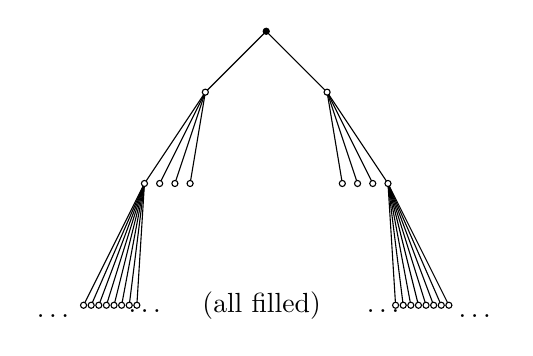
\begin{tikzpicture}[scale=1.1]

\newcommand\X{20pt}
\newcommand\Y{-20pt}

\newcommand\ADDYA{-10pt}
\newcommand\ADDYB{-30pt}

\draw (0*\X, 0*\Y) -- (-1*\X, 1*\Y);
\draw (0*\X, 0*\Y) -- ( 1*\X, 1*\Y);

\draw[fill=black] (0*\X, 0*\Y) circle (1pt); 
%% 

\draw (-1*\X, 1*\Y) -- (-1.25*\X, \ADDYA + 2*\Y);
\draw (-1*\X, 1*\Y) -- (-1.5*\X, \ADDYA + 2*\Y);
\draw (-1*\X, 1*\Y) -- (-1.75*\X, \ADDYA + 2*\Y);
\draw (-1*\X, 1*\Y) -- (-2*\X, \ADDYA + 2*\Y);
\draw (1*\X, 1*\Y) -- (1.25*\X, \ADDYA + 2*\Y);
\draw (1*\X, 1*\Y) -- (1.5*\X, \ADDYA + 2*\Y);
\draw (1*\X, 1*\Y) -- (1.75*\X, \ADDYA + 2*\Y);
\draw (1*\X, 1*\Y) -- (2*\X, \ADDYA + 2*\Y);

\draw[fill=white] (-1*\X, 1*\Y) circle (1pt); 
\draw[fill=white] (1*\X, 1*\Y) circle (1pt); 
%%

\draw(-2*\X, \ADDYA + 2*\Y) -- (-2.125*\X, \ADDYB + 3*\Y);
\draw(-2*\X, \ADDYA + 2*\Y) -- (-2.25*\X, \ADDYB + 3*\Y);
\draw(-2*\X, \ADDYA + 2*\Y) -- (-2.375*\X, \ADDYB + 3*\Y);
\draw(-2*\X, \ADDYA + 2*\Y) -- (-2.5*\X, \ADDYB + 3*\Y);
\draw(-2*\X, \ADDYA + 2*\Y) -- (-2.625*\X, \ADDYB + 3*\Y);
\draw(-2*\X, \ADDYA + 2*\Y) -- (-2.75*\X, \ADDYB + 3*\Y);
\draw(-2*\X, \ADDYA + 2*\Y) -- (-2.875*\X, \ADDYB + 3*\Y);
\draw(-2*\X, \ADDYA + 2*\Y) -- (-3*\X, \ADDYB + 3*\Y);
\draw(2*\X, \ADDYA + 2*\Y) -- (2.125*\X, \ADDYB + 3*\Y);
\draw(2*\X, \ADDYA + 2*\Y) -- (2.25*\X, \ADDYB + 3*\Y);
\draw(2*\X, \ADDYA + 2*\Y) -- (2.375*\X, \ADDYB + 3*\Y);
\draw(2*\X, \ADDYA + 2*\Y) -- (2.5*\X, \ADDYB + 3*\Y);
\draw(2*\X, \ADDYA + 2*\Y) -- (2.625*\X, \ADDYB + 3*\Y);
\draw(2*\X, \ADDYA + 2*\Y) -- (2.75*\X, \ADDYB + 3*\Y);
\draw(2*\X, \ADDYA + 2*\Y) -- (2.875*\X, \ADDYB + 3*\Y);
\draw(2*\X, \ADDYA + 2*\Y) -- (3*\X, \ADDYB + 3*\Y);

\draw[fill=white] (-1.25*\X, \ADDYA + 2*\Y) circle (1pt);
\draw[fill=white] (-1.5 *\X, \ADDYA + 2*\Y) circle (1pt);
\draw[fill=white] (-1.75*\X, \ADDYA + 2*\Y) circle (1pt);
\draw[fill=white] (-2*\X, \ADDYA + 2*\Y) circle (1pt);
\draw[fill=white] (1.25*\X, \ADDYA + 2*\Y) circle (1pt);
\draw[fill=white] (1.5 *\X, \ADDYA + 2*\Y) circle (1pt);
\draw[fill=white] (1.75*\X, \ADDYA + 2*\Y) circle (1pt);
\draw[fill=white] (2*\X, \ADDYA + 2*\Y) circle (1pt);

%%

\draw[fill=white] (-2.125*\X, \ADDYB + 3*\Y) circle (1pt);
\draw[fill=white] (-2.25*\X, \ADDYB + 3*\Y) circle (1pt);
\draw[fill=white] (-2.375*\X, \ADDYB + 3*\Y) circle (1pt);
\draw[fill=white] (-2.5*\X, \ADDYB + 3*\Y) circle (1pt);
\draw[fill=white] (-2.625*\X, \ADDYB + 3*\Y) circle (1pt);
\draw[fill=white] (-2.75*\X, \ADDYB + 3*\Y) circle (1pt);
\draw[fill=white] (-2.875*\X, \ADDYB + 3*\Y) circle (1pt);
\draw[fill=white] (-3*\X, \ADDYB + 3*\Y) node[anchor=north east]{\ldots} circle (1pt);
\draw[fill=white] (2.125*\X, \ADDYB + 3*\Y) circle (1pt);
\draw[fill=white] (2.25*\X, \ADDYB + 3*\Y) circle (1pt);
\draw[fill=white] (2.375*\X, \ADDYB + 3*\Y) circle (1pt);
\draw[fill=white] (2.5*\X, \ADDYB + 3*\Y) circle (1pt);
\draw[fill=white] (2.625*\X, \ADDYB + 3*\Y) circle (1pt);
\draw[fill=white] (2.75*\X, \ADDYB + 3*\Y) circle (1pt);
\draw[fill=white] (2.875*\X, \ADDYB + 3*\Y) circle (1pt);
\draw[fill=white] (3*\X, \ADDYB + 3*\Y) node[anchor=north west]{\ldots} circle (1pt);

\draw (0*\X, \ADDYB + 3*\Y)node{\ldots \ \ \ \ (all filled) \ \ \ \ \ldots};



\end{tikzpicture}}
  \hspace{5pt}
  \subfloat[\LSEQ tree filled using monotonic editing.]
  [\label{fig:monotoniclseq} \LSEQ tree filled using monotonic editing.]
  {
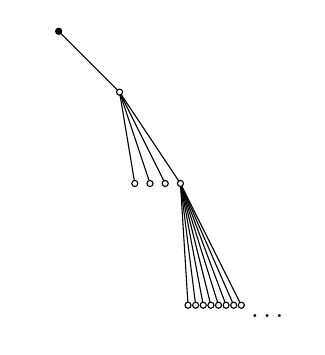
\begin{tikzpicture}[scale=1.1]

\newcommand\X{20pt}
\newcommand\Y{-20pt}

\newcommand\ADDYA{-10pt}
\newcommand\ADDYB{-30pt}

\draw (-0.5*\X, 0*\Y); %% spacing

\draw (0*\X, 0*\Y) -- ( 1*\X, 1*\Y);

\draw[fill=black] (0*\X, 0*\Y) circle (1pt); 
%% 

\draw (1*\X, 1*\Y) -- (1.25*\X, \ADDYA + 2*\Y);
\draw (1*\X, 1*\Y) -- (1.5*\X, \ADDYA + 2*\Y);
\draw (1*\X, 1*\Y) -- (1.75*\X, \ADDYA + 2*\Y);
\draw (1*\X, 1*\Y) -- (2*\X, \ADDYA + 2*\Y);

\draw[fill=white] (1*\X, 1*\Y) circle (1pt); 
%%

\draw(2*\X, \ADDYA + 2*\Y) -- (2.125*\X, \ADDYB + 3*\Y);
\draw(2*\X, \ADDYA + 2*\Y) -- (2.25*\X, \ADDYB + 3*\Y);
\draw(2*\X, \ADDYA + 2*\Y) -- (2.375*\X, \ADDYB + 3*\Y);
\draw(2*\X, \ADDYA + 2*\Y) -- (2.5*\X, \ADDYB + 3*\Y);
\draw(2*\X, \ADDYA + 2*\Y) -- (2.625*\X, \ADDYB + 3*\Y);
\draw(2*\X, \ADDYA + 2*\Y) -- (2.75*\X, \ADDYB + 3*\Y);
\draw(2*\X, \ADDYA + 2*\Y) -- (2.875*\X, \ADDYB + 3*\Y);
\draw(2*\X, \ADDYA + 2*\Y) -- (3*\X, \ADDYB + 3*\Y);


\draw[fill=white] (1.25*\X, \ADDYA + 2*\Y) circle (1pt);
\draw[fill=white] (1.5 *\X, \ADDYA + 2*\Y) circle (1pt);
\draw[fill=white] (1.75*\X, \ADDYA + 2*\Y) circle (1pt);
\draw[fill=white] (2*\X, \ADDYA + 2*\Y) circle (1pt);

%%

\draw[fill=white] (2.125*\X, \ADDYB + 3*\Y) circle (1pt);
\draw[fill=white] (2.25*\X, \ADDYB + 3*\Y) circle (1pt);
\draw[fill=white] (2.375*\X, \ADDYB + 3*\Y) circle (1pt);
\draw[fill=white] (2.5*\X, \ADDYB + 3*\Y) circle (1pt);
\draw[fill=white] (2.625*\X, \ADDYB + 3*\Y) circle (1pt);
\draw[fill=white] (2.75*\X, \ADDYB + 3*\Y) circle (1pt);
\draw[fill=white] (2.875*\X, \ADDYB + 3*\Y) circle (1pt);
\draw[fill=white] (3*\X, \ADDYB + 3*\Y) node[anchor=north west]{\ldots} circle (1pt);



\end{tikzpicture}}
  \hspace{5pt}
  \subfloat[Worst case \LSEQ tree.]
  [\label{fig:worstlseq} Worst case \LSEQ tree.]
  {
\begin{tikzpicture}[scale=1.]

\newcommand\X{20pt}
\newcommand\Y{-20pt}

\newcommand\ADDYA{-10pt}
\newcommand\ADDYB{-30pt}

%\draw (-3*\X, 0*\Y); %% spacing

\draw (0*\X, 0*\Y) -- ( 1*\X, 1*\Y);

\draw[fill=black] (0*\X, 0*\Y) circle (1pt); 
%% 

\draw (1*\X, 1*\Y) -- (2*\X, \ADDYA + 2*\Y);

\draw[fill=white] (1*\X, 1*\Y) circle (1pt); 
%%

\draw(2*\X, \ADDYA + 2*\Y) -- (3*\X, \ADDYB + 3*\Y);


\draw[fill=white] (2*\X, \ADDYA + 2*\Y) circle (1pt);

%%

\draw[fill=white] (3*\X, \ADDYB + 3*\Y) node[anchor=north west]{\ldots} circle (1pt);



\end{tikzpicture}}
  \caption{\label{fig:complexity} \LSEQ tree filled with the studied editing
    behaviors and in the worst case.}
\end{figure*}


In text editing, most of the editing behaviors can be empirically summarized as
a composition of two basic editing behaviors:
\begin{itemize}
\item The random editing behavior where the author inserts new elements at what
  appears random positions in the sequence. For instance, this behavior mostly
  arises when syntactic corrections are performed, e.g. the author writes
  \texttt{QWETY} and realizes that the \texttt{R} is missing. She adds the
  missing character in a second time.
\item The monotonic editing behavior where the author repeatedly inserts new
  elements between the last inserted element and an adjacent element (after or
  before exclusively). For instance, when an author writes \texttt{QWERTY}, she
  generally starts from the first character \texttt{Q} to the last letter of the
  word \texttt{Y}. On the opposite, there exist documents mainly edited at the
  beginning
  (e.g. \url{http://en.wikipedia.org/wiki/Template_talk:Did_you_know}~\cite{nedelec2013lseq}). This
  behavior characterizes both left-to-right and right-to-left editing.
\end{itemize}

\noindent As a consequence, we focus on the space complexity analysis of \LSEQ
to random and monotonic editing behaviors. It is worth noting that monotonic
editing behavior represents an unfavorable case since it tends to unbalance the
underlying tree storing the replicated sequence. As soon as the participants
start to edit at different positions -- which is closer from a real-life use
case -- the tree becomes more balanced.
The analysis does not include an average case, for it requires knowing
the average distribution of the position of edits performed by humans which is
obviously complex.

\noindent The complexity analysis also includes a worst case analysis. In the
worst case, each new identifier is bigger than the previous one. To produce such
worst case in \LSEQ, the insertions must saturate the small gap left between
identifiers (see Lines~\ref{line:plus} and~\ref{line:minus} of
Algorithm~\ref{algo:allocpath}). The editing behavior that produces such worst
case with \LSEQ is the following:
\begin{inparaenum}[(1)]
\item The user types \texttt{A} followed by \texttt{B}. The gap left between
  \texttt{A} and \texttt{B} corresponds to the $boundary$ (see
  Line~\ref{line:boundary} of Algorithm~\ref{algo:allocpath});
\item The user types $boundary$ characters between the two lastly inserted
  characters. At least the last identifier has grown;
\item Repeat the second step.
\end{inparaenum}
The editing behavior that produces such worst case with the
state-of-the-art~\cite{preguica2009commutative, weiss2009logoot} is the
following:
\begin{inparaenum}[(1)]
\item The user types a character at the beginning of the document;
\item Repeat the first step.
\end{inparaenum}

The complexity analysis depends of the chosen structure to represent the
replica. In this section, we focus on a tree structure but other structures
(e.g. lists~\cite{weiss2009logoot}) exposing different tradeoffs could be
used. Nevertheless, the space complexity of identifiers -- the main contribution
of \LSEQ{} -- stays the same regardless of the chosen structure.

\paragraph{Space complexity.}

We distinguish the space complexity of each identifier from the space complexity
of the tree. The former is important since it directly impacts the communication
complexity, for that each identifier is broadcast to all editors; The latter is
important since it represents the replicated document stored locally by each
editor.

As stated in Section~\ref{subsec:lseqallocation}, paths require
$\mathcal{O}(e^2)$ bits to be encoded, where $e$ is the depth of the element in
the tree. Fortunately, the depth is upper-bounded depending on the editing
behavior that filled the exponential tree.

The random editing behavior fills the tree at random. The repeated insertions
progressively fill the gaps in the tree without favoring any position in the
document. Over insertions, the lowest branches of the tree become filled of
elements and the depth of the tree grows slowly (see
Figure~\ref{fig:randomlseq}). Thus, the random editing behavior balances the
tree. Being exponential, the tree stores
$\textstyle\sum\nolimits_{i=1}^{k}{2^{(i^2-i)/2}}$ elements, where $k$ is the
depth of the tree. The depth of paths is upper-bounded by
$\mathcal{O}(\sqrt{\log I})$ concatenations, where $I$ is the number of
insertions. Since paths require $\mathcal{O}(e^2)$ bits to encode, paths have an
optimal logarithmic space complexity $\mathcal{O}(\log I)$. This result applies
to all variable-size identifier allocators~\cite{preguica2009commutative,
  weiss2009logoot}. A tree structure factorizes common parts of
identifiers. Overall, the space complexity is not the sum of identifiers but
$\mathcal{O}(I\log I)$.

The monotonic editing behavior fills only one branch of the tree (see
Figure~\ref{fig:monotoniclseq}). Yet, since the maximum arity grows over depths, the
growth of the tree tends decelerate over insertions. The tree stores up till
$2^{e+1}-1$ elements, where $e$ is the depth of the tree. Hence, the number of
concatenation composing a path is $\mathcal{O}(\log I)$, where $I$ is the number
of insertions. Since the binary representation of paths increases quadratically,
the space complexity of paths taken individually is upper-bounded by
$\mathcal{O}((\log I)^2)$.  Overall, the space complexity of the tree remains
upper-bounded by $\mathcal{O}(I\log I)$.

In the worst case, each insertion increases the depth of the tree. Thus, after
$I$ insertions, the tree comprises $e$ elements, where $e$ is the depth of the
tree (see Figure~\ref{fig:worstlseq}). The space complexity of paths grows
quadratically and each new allocated path contains the full tree. For instance,
the first allocated path is [$31$], the second one is [$31.63$], the third one
is [$31.63.127$], etc.  Overall, the space complexity of the tree is
$\mathcal{O}(I^2)$ too.

\begin{table*}
  \caption{\label{table:lseqspace}
    Upper bounds on space complexity of \LSEQ, Logoot and Treedoc. Where
    $I$ is the number of insertions performed on the replicated sequence.}
  \centering
  
\begin{tabularx}{0.6\textwidth}{@{}Xcc@{}}

  \toprule
  \textsc{Editing behavior} & \multicolumn{2}{c}{\textsc{Space}} \\ \cmidrule{2-3} 
                   & \textsc{Identifier} & \textsc{Sequence} \\ \midrule
  Random editing & $\mathcal{O}(\log I)$ & $\mathcal{O}(I\log I)$ \\
  Monotonic editing & $\mathcal{O}((\log I)^2)$ & $\mathcal{O}(I \log I)$ \\
  Worst case & $\mathcal{O}(I^2)$ & $\mathcal{O}(I^2)$ \\ \bottomrule
\end{tabularx}

\end{table*}

Table~\ref{table:lseqspace} summarizes the space complexity of \LSEQ. In
particular, the expected growth of identifiers is bounded between an optimal
logarithm and a polylogarithm, hence, a sub-linear upper bound compared to the
number of insertions. To provide such improvement, \LSEQ sacrifices on its worst
case complexity that becomes quadratic. However, this worst case is made
difficult to produce, for the two sub-allocations functions with antagonist
designs settle each other's deficiency. Furthermore, if a malicious user tries
to produce the worst case, the difference in complexity makes it easy to detect,
hence, to handle. Table~\ref{table:lseqspace} also shows that compared to
state-of-the-art, \LSEQ significantly improves the identifiers size but exposes
a small overhead on the full structure, i.e. from $\mathcal{O}(I)$ to
$\mathcal{O}(I\log I)$. The tradeoff is beneficial since the communication
complexity of editors inherits from the improvement: as shown in
Algorithm~\ref{algo:crdtabstract}, each identifier is broadcast to all editors.

\paragraph{Time complexity.}

Time complexity provides insights about the performance evolution of each
operation over insertions. They are divided between their local execution and
their remote integration.  Similarly to the space complexity, the analysis
focuses on two editing behaviors (random and monotonic) to which we add the
worst case.

The local insert operation simply consists in building a new path according to
two adjacent paths. Therefore, it depends of the depths of the latter which grow
depending on the editing behavior. Since the random editing behavior, the
monotonic editing behavior, and the worst case respectively lead to a depth
growth upper-bounded by $\mathcal{O}(\sqrt{\log I})$, $\mathcal{O}(\log I)$ and
$\mathcal{O}(I)$, the time complexity of the local part of the insert operation
follows: $\mathcal{O}(\sqrt{\log I})$, $\mathcal{O}(\log I)$ and
$\mathcal{O}(I)$.

The local delete operation simply broadcasts the identifier of the element to
remove to all participants. Hence, the time complexity is constant
$\mathcal{O}(1)$ regardless of the editing behavior.

Both the remote insert and delete operations perform the same instructions to
integrate the received result. Consequently, they have an identical time
complexity. Random, monotonic, and worst case editing behaviors respectively
lead to $\mathcal{O}(\sqrt{\log I})$, $\mathcal{O}(\log I)$ and $\mathcal{O}(I)$
levels in the exponential tree structure. Since the children of each node are
ordered by path, we perform binary searches recursively until we find the
leaf. During binary searches, the delete operation removes the nodes it explores
if they, or their children, do not contain at least another element. For
instance, considering two elements associated to the following paths: [$3.1$]
and [$3.1.2$]. If one deletes the first element, the path is kept since the path
labeled by $3$ then $1$ is still required for the second element. Then, if one
deletes the second element and the node containing it has no children, the path
and nodes are truly removed. The complexity of a binary search depends of the
level $l$ at which it is performed: $\mathcal{O}(\log 2^l)$. Repeated binary
searches lead to the upper bound
$\mathcal{O}(\textstyle\sum\nolimits_{i=1}^{e}(\log 2^i))$, where $e$ is the
depth of the tree. Replacing the depth $e$, upper bounds on time complexity are
$\mathcal{O}(\log I + \sqrt{log I})$, $\mathcal{O}((\log I)^2+\log I)$, and
$\mathcal{O}(I)$ for random, monotonic, and worst case editing behaviors
respectively. In the worst case, the algorithms perform one comparison per
element, i.e. per level, in the tree until they reach the deepest leaf.


\begin{table*}
  \caption{\label{table:lseqtime}
    Upper bounds on time complexity of \LSEQ. Where $I$ is the number of 
    insertions performed on the replicated sequence.}
  \centering
  
\begin{tabularx}{0.455\textwidth}{@{}Xcccc@{}}
  \toprule
  \textsc{Editing} & \multicolumn{4}{c}{\textsc{Time}} \\
  \textsc{behavior} & \multicolumn{2}{c}{\textsc{Local}} & \multicolumn{2}{c}{\textsc{Remote}} \\ \cmidrule(r){2-3} \cmidrule(l){4-5}
  & \textsc{ins} & \textsc{del} & \ \ \ \ \textsc{ins} & \textsc{del}  \\ \midrule
  Random & $\mathcal{O}(\sqrt{\log I})$ & $\mathcal{O}(1)$ & \multicolumn{2}{c}{$\mathcal{O}(\log I + \sqrt{\log I})$} \\
  Monotonic & $\mathcal{O}(\log I)$ & $\mathcal{O}(1)$ & \multicolumn{2}{c}{$\mathcal{O}((\log I)^2 +\log I)$} \\
  Worst case & $\mathcal{O}(I)$ & $\mathcal{O}(1)$ & \multicolumn{2}{c}{$\mathcal{O}(I)$} \\ \bottomrule
\end{tabularx}


\end{table*}

To interface the user's view of the document with the underlying replicated
sequence, an additional lookup operation is necessary. Its goal is to retrieve
the identifier of the element at the specified index in the sequence, and
converse. Since the structure is a tree, this access is not direct.

To consistently manage the translation between sequence structure and the tree
structure, the latter stores with each node the number of elements included in
its sub-trees. Each insertion and removal updates these counters as they explore
a path. Then, processing an index comes down to count the number of elements in
the siblings of explored nodes starting from the beginning or the end of the
sequence. Unfortunately, it can be costly depending on the editing behavior that
filled the tree.

The random editing behavior leads to an exponential tree of depth bounded by
$\mathcal{O}(\sqrt{\log I})$. In such a case, a very small portion of the whole
tree will be explored. The upper bound happens when the explored nodes are
exactly in the middle of its siblings, for it forces to check at least half of
these sibling per depth. Since each node stores twice as much children as its
parents. The number of siblings to check doubles at each depth. Overall, the sum
of these siblings is equal to the number of node at the deepest level, which is
$\mathcal{O}(2^{\sqrt{\log I}})$ elements. 

From an identical reasoning, the lookup operation after monotonic editing --
which also constitutes the worst case for this operation -- is upper-bounded by
$\mathcal{O}(I)$. Indeed, only one branch is filled and explored. The counters
become useless since all nodes but one have only one child. The exploration
directly ends up in the deepest level containing $\mathcal{O}(2^{\log_2 I})$
elements where half of them must be checked leading to
$\mathcal{O}(I)$.

\begin{table}
  \caption{\label{table:lseqlookup}
    Upper bounds on time complexity of the lookup on a \LSEQ structure.
    Where $I$ is the number of insertions performed on the replicated sequence.}
  \centering
  
\begin{tabularx}{0.6\textwidth}{@{}Xc@{}}
  \toprule
  \textsc{Editing behavior} & \textsc{Time} \\
  & \ \ \ \ \ \ \ \ \ \textsc{Look-up} \ \ \ \ \ \ \ \ \ \\ \midrule
  Random editing & $\mathcal{O}(2^{\sqrt{\log I}})$ \\
  Monotonic editing & $\mathcal{O}(I)$ \\
  Worst case & $\mathcal{O}(I)$ \\ \bottomrule
\end{tabularx}


\end{table}

Tables~\ref{table:lseqtime} and~\ref{table:lseqlookup} summarize the time
complexity of operations. The exponential tree structure leads to efficient
update operations. Its drawback lies in the lookup operation making the link
between the sequence and the tree. In particular, monotonic editing leads to the
worst case scenario where the access grows linearly. Fortunately,
\begin{inparaenum}[(i)]
\item the view should not be updated if the index of the change falls outside
  the user's visibility window. Thus, the lookup can stop earlier if it explores
  the tree outside the scope;
\item keeping fast accesses to the newest path and its adjacent paths removes
  the cost of the lookup, for the repeated insertions -- if monotonic -- alone
  can maintain these fast accesses up-to-date.
\end{inparaenum}

\paragraph{Summary.}

The complexity analysis reveals the improvements brought by \LSEQ as well as
their cost.  \LSEQ sacrifices on its worst case complexity to improve on other
editing behaviors that are considered more likely to happen in collaborative
editing. The most important result is the polylogarithmic space complexity of
identifiers, for it applies on communication complexity. In comparison,
state-of-the-art allocators~\cite{preguica2009commutative, weiss2009logoot} only
provided linearly upper-bounded identifiers. Other analysis such as the local
space consumed by the replicated structure, and the time complexity of provided
operations shows that the tree as replicated structure is
efficient. Nonetheless, based on preferences, one could choose an array -- as a
flat version of the tree -- to improve the performance of operations at the cost
of increased memory usage~\cite{weiss2009logoot}.  Section~\ref{sec:experiments}
validates our complexity analysis on experiments. The next section describes the
other components necessary to build a decentralized collaborative editor that
scales.

%%% Local Variables: 
%%% mode: latex
%%% TeX-master: "../paper"
%%% End: 
\section{Experiments}
\label{sec:experiments}

The objective of this experiment section is threefold:
\begin{itemize}
\item To show the evolution of the average neighborhood size of members of an
  editing session. Using \SPRAY, we expect a logarithmic growth compared to the
  global size of the network.
\item To confirm the space complexity of the identifiers generated by \LSEQ. On
  the common monotonic editing behavior, we expect a polylogarithmic growth
  compared to the document size.
\item To show that both the identifier size and neighborhood size impact the
  traffic. Since the former grows polylogarithmically, and the latter grows
  logarithmically, we expect the traffic to scale in terms of number users and
  number of operations.
\end{itemize}

We conducted the experiments using a Javascript implementation directly usable
within modern web browsers\footnote{https://github.com/Chat-Wane/CRATE}. The
experiments ran on the \emph{Grid'5000} testbed involving uptil 601 instances of
the editor distributed among 101 machines.

\ \\ 

\begin{figure}
  \centering
  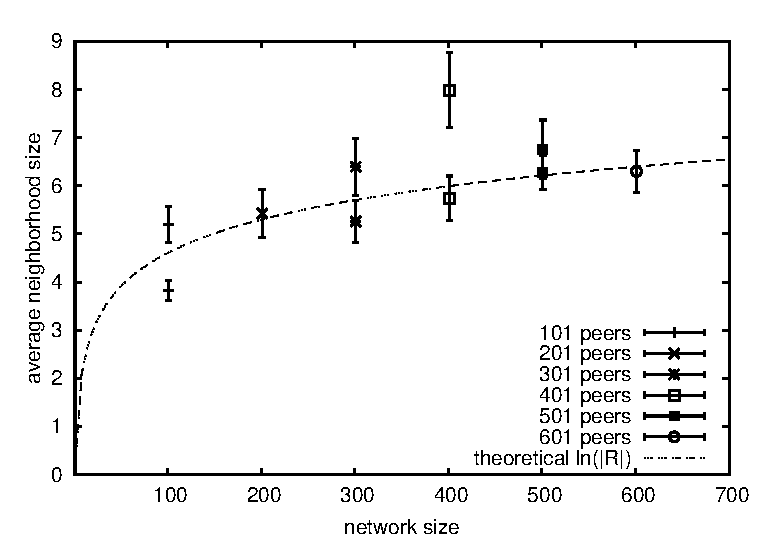
\includegraphics[width=0.475\textwidth]{./img/partialview.eps}
  \caption{\label{fig:partialview} Average neighborhood size of each peer over
  the global network size.}
\end{figure}

\begin{asparadesc}
\item [Objective:] To show the evolution of the average neighborhood size of
  members of an editing session. The \SPRAY protocol aims to provide a
  logarithmically scaling neighborhood compared to the global network
  size. Furthermore, the protocol builds a dynamic network where the load is
  balanced among members.
\item [Description:] During a run, peers dynamically modify their
  neighborhood. Each peer periodically reports its neighborhood size. Then, we
  average all these values and measure the variance. The average value defines
  how connected is a member to the network, impacting (among other) on the
  information dissemination efficiency. The variance defines how spread are the
  values; a small value means a good load balancing among members. Runs comprise
  from 101 members to 601 members with 100 members increments, i.e., 6 different
  runs.  The first member creates the editing session which is progressively
  joined by the other writers (1 joiner per 5 seconds). Each member starts
  sharing the document as soon as its joining. Hence, outsiders can join the
  network through one of them chosen at random.
\item [Results:] Figure~\ref{fig:partialview} shows the results of this
  experiment. The figure displays the network size on the x-axis and the average
  neighborhood size on the y-axis. It shows the average value of each experiment
  along with the theoretical expectation: a natural logarithm on the global
  network size. Each average value also carries the variance measurement. As
  expected, we observe that the average neighborhood size grows logarithmically
  compared to the size of the network despite being scattered around the
  theoretical curve. Figure~\ref{fig:partialview} also shows that the variance
  is small around the average values. Thus, members have an even neighborhood
  size. In other terms, the load is well-balanced among members when they need
  to disseminate information to the whole network. At the opposite of
  centralized solutions, it builds a topology where no member is more important
  than another in term of connectivity. As such, the network is more resilient
  to random crashes or unexpected departures.
\item [Reasons:] When an outsider wants to join the editing session, it picks a
  random sharer as first contact. \SPRAY assumes that the neighborhood size of
  this particular member is already logarithmic compared to the network
  size. Therefore, it uses this assumption to create additional connections that
  increase logarithmically in number. Yet, the averages neighborhood size does
  not follow exactly the theoretical expectation curve. Indeed, the number of
  neighbors of each member strongly depends of the first contact. However, the
  specific average value is not necessarily reached, especially considering
  that, while the theoretical expectation is a floating number, the neighborhood
  size belongs to the integers. This fact also impacts the variance. Indeed, the
  \SPRAY protocol exchanges the neighborhood of member over time. During the
  exchanges, it aims to balance the neighborhood size of each peer. Yet, the
  average value may not be an integer value. Therefore, the neighborhood size of
  the members constantly fluctuates around the average value.
\end{asparadesc}

\ \\

\begin{figure}
  \centering
  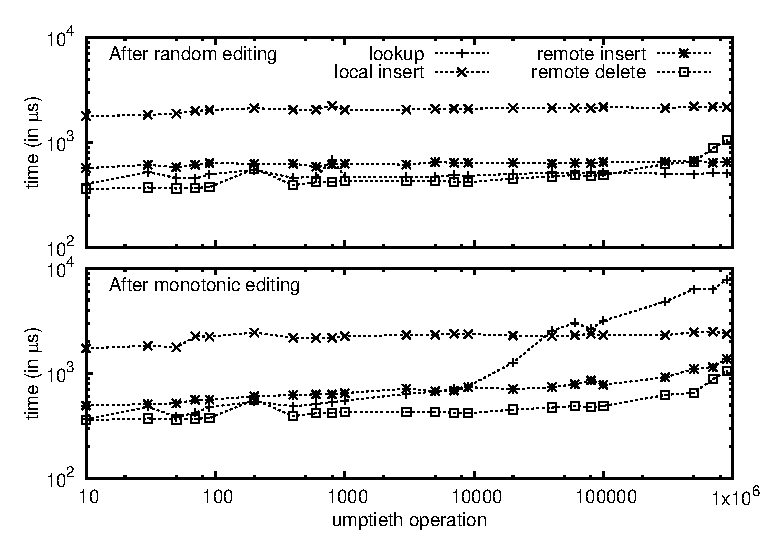
\includegraphics[width=0.475\textwidth]{./img/bench.eps}
  \caption{\label{fig:bench} Time performance of operations.}
\end{figure}

\begin{asparadesc}
\item [Objective:] To confirm the time complexity of the operations of
  \LSEQ.
\item [Description:] This experiment involves only one user performing
  operations on its local copy. The benchmark ran on a MacBook Pro with 2.5 GHz
  Intel Core i5, with \emph{Node.js 4.1.1 on Darwin 64-bit}. Yet, we are more
  interested in tendencies than absolute values. Indeed, since Javascript does a
  lot of optimisation on-the-fly, performances are better than they appear in
  this benchmark. To expose the behavior of operations individually, we limit
  the buit-in optimisation to the maximum.
\item [Results:]
\item [Reasons:]
\end{asparadesc}

\ \\

\begin{figure}
  \centering
  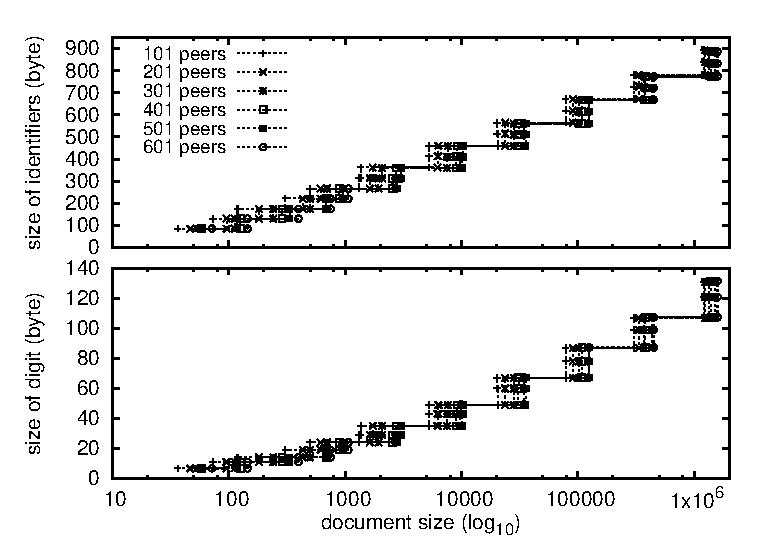
\includegraphics[width=0.475\textwidth]{./img/identifiers.eps}
  \caption{\label{fig:identifiers} Average identifiers size.}
\end{figure}

\begin{asparadesc}
\item [Objective:] To confirm the space complexity of the identifiers generated
  by \LSEQ. On the common monotonic editing behavior, we expect a
  polylogarithmic growth compared to the document size.
\item [Description:] The executions follow the previous experiment about the
  neighborhood size. Thus, the experimentation comprises 6 runs with networks
  including 101, 201, 301, 401, 501, 601 members. The editing session members
  are repeatedly inserting new characters at the end of the document. The rate
  of these operation is 100 operations per second distributed among
  members. Thus, the experiment involving 101 members forces each member to
  perform 1 insertion per second, while the experiment involving 601 members
  forces each member to perform 1 insertion every 6 seconds. During the runs,
  each author reports the byte-size of newly generated identifiers along with
  the byte-size of its path in the exponential tree. \TODO{site, counter,
    starting values of the exponential tree}.
\item [Results:] Figure~\ref{fig:identifiers} shows the result of this
  experimentation. The x-axis denotes the document size (which is equivalent to
  the number of insert operations since the members do not perform removals) on
  a decimal logarithmic scale. Thus, the document grows from empty to above a
  million characters. The y-axis of the top part of the figure denotes the
  byte-size of the identifiers while the bottom part of the figure denotes the
  byte-size of the path only. First, we observe that all plots are very close
  from each other. Hence, the size of identifiers does not depend of the number
  of participants. Second, we observe that the identifiers grows
  polylogarithmically compared to the size of the document. Indeed, the bottom
  part of Figure~\ref{fig:identifiers} shows that the increment step of the
  generated paths is slowly increasing during the experiment. It empirically
  exposes a small surlinear behavior when the x-axis is on a logarithmic
  scale. Hence the polylogarithmic curve. Finally, we can observe that \LSEQ
  generates paths the size of which is small comparatively to the whole
  identifier that includes site identifiers and counters to guarantee
  uniqueness.
\item [Reasons:] The curves of the byte-size are close because the identifiers
  of \LSEQ do not depend of whom created it nor the number of authors involved
  in the document editing. They only depend of the position of insertions which
  globally corresponds to the editing behavior. In this case, the highlighted
  editing behavior is a monotonic left-to-right editing, i.e., repeated
  insertions at the end of the document. This kind of behavior tends to
  unbalance the tree by filling only one branch per level of the
  tree. Fortunately, since the tree exponentially grows (each element has twice
  as much children as its parent), the path growth slowly decreases over
  insertions. Nevertheless, it costs one additional bit to encode each
  concatenation of the path, hence the path growth on the bottom part of the
  figure. The identifiers are much heavier than the path they carry because they
  also includes a list of pairs to guarantee the uniqueness of identifiers and a
  global total order. Each member generates its own globally unique identifier
  (with high probability) without relying on any remote service. As such, they
  require large identifiers that does not collide with remote members.
\end{asparadesc}

\ \\

\begin{figure}
  \centering
  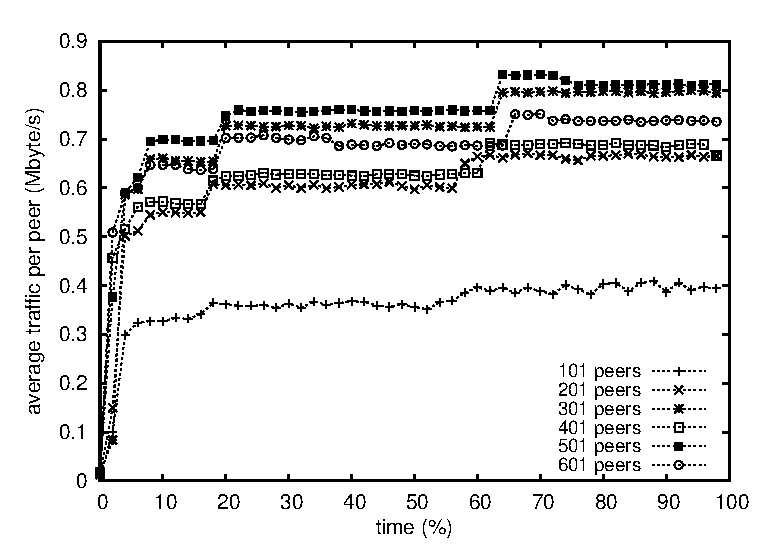
\includegraphics[width=0.475\textwidth]{./img/traffic.eps}
  \caption{\label{fig:traffic} Average traffic per second at each peer
    during the experiments.}
\end{figure}

\begin{asparadesc}
\item [Objective:] To show that both the identifier size and neighborhood size
  impact the traffic. Since the former grows polylogarithmically, and the latter
  grows logarithmically, we expect the traffic to scale in terms of number users
  and number of operations.
\item [Description:] As for prior experiments, this experimentation concerns
  networks from 101 members to 601 members, each coauthoring a document of over
  a million of characters. Figure~\ref{fig:partialview} displays the average
  neighborhood size of members of each run. Figure~\ref{fig:identifiers}
  displays the identifiers size of each run. This experiment measure average
  traffic of members in MByte per second.
\item [Results:] Figure~\ref{fig:traffic} shows the result of this experiment.
\item [Reasons:]
\end{asparadesc}

%%% Local Variables:
%%% mode: latex
%%% TeX-master: "../paper"
%%% End:

\section{Related Work}
\label{sec:relatedwork}

Real-time distributed collaborative editors consider multiple participants, each
hosting a copy -- or replica -- of a shared sequence of characters. Participants
can update their copy by inserting or deleting a character at any time. Then,
the editor eventually delivers the change to all participants. Finally, each
editor integrates the received operations~\cite{saito2005optimistic}. Strong
eventual consistency~\cite{bailis2013eventual, shapiro2011comprehensive,
  sun1998achieving} requires that editors integrating a same set of operations
converge to an equivalent state, i.e. users see the same document. Furthermore,
operations must preserve the intention of users, i.e. effects observed at
generation time must be re-observed at integration time regardless of concurrent
operations. Finally, the integration order of operations must follow the
\emph{happen before} relationship~\cite{lamport1978time} stated at generation.

\noindent Four complexities characterize editors:
\begin{itemize}[noitemsep, leftmargin=*]
\item Generation time: complexity to generate locally an operation.
\item Integration time: complexity to execute remotely an operation.
\item Space complexity: complexity to store a local copy of the shared sequence.
\item Communication complexity: complexity of messages transiting the network.
\end{itemize}
Solving scalability issues requires finding a balance between communication,
space and time complexities %  Among others, the communication complexity is the
% most discriminant and depends of metadata required to ensure strong eventual
% consistency as well as messages dissemination in the network.
where the communication complexity complexity plays the most important role. The
challenge consists in providing a sublinear upper bound on communication
complexity without making other complexities impracticable.

% It requires $\mathcal{O}(m.\ln{R})$ where ($\ln{R}$) is a minimal multiplicative
% factor induced by the broadcasting mechanism which depends of the session size
% $R$ including both readers and writers; where $m$ is the message embedding
% metadata necessary to maintain consistency. To scale, the space complexity of
% these metadata must be sublinear.

\begin{asparadesc}
\item [Operational transformation] (OT) allows building both centralized and
  decentralized real-time editors. At generation, the processing time of
  operations is constant. At integration, OT transforms the received operations
  against concurrent ones which were generated on the same state. An integration
  algorithm such as COT~\cite{sun2009contextbased} or
  SOCT2~\cite{vidot2000copies} along with transformation functions (ensuring
  transformation properties) guarantee a consistent model. The integration time
  depends of concurrency and differs among the algorithms.  For instance, COT's
  integration time complexity is exponential. It can reduce it to linear at the
  expense of space complexity. SOCT2's integration time complexity is quadratic.
  Whatever the trade-off, OT's integration algorithms rely on concurrency
  detection which costs, at least, a state
  vector~\cite{charronbost1991concerning} the size of which grows linearly
  compared to the number of members $W$ who ever participated in the
  authoring. Since each message embeds such vector, decentralized OT approaches
  are not practicable in large groups subject to churn where people join and
  leave the network frequently and freely.  As for space complexity, OT
  approaches require an historic of operations $H$, each operation being linked
  to their state vector, hence $\mathcal{O}(W.H)$. Such monotonically growing
  historic can be cut at the price of consensus which, once again, does not
  scale~\cite{mostefaoui2015signature}. Thus, OT approaches are the best in
  humble confined environment like local area networks. However, their
  performance degrades when the network size grows and becomes unpredictable
  like wide area networks.

\item [Conflict-free replicated data types~\cite{shapiro2011comprehensive,
    shapiro2011conflict}] (CRDTs) for sequences constitute the latter approaches
  which solve concurrent cases by providing commutative, associative, and
  idempotent operations. As such, and compared to OT, the causality tracking
  cost is drastically reduced since it only requires tracking semantically
  related operations. For instance, the removal of a particular element must
  follow its insertion. The commutative property of operations ensures the
  consistency of the system. CRDTs provide commutativity by associating a unique
  and immutable identifier to each element. Defining a total order among the
  identifiers allows retrieving the sequence of characters.

  CRDTs propose interesting trade-offs since they can balance complexities
  depending on the type of structure that represents the document.  In
  particular, increasing the generation time of operations to decrease the
  integration time is profitable since an operation generated once is
  re-executed many times. Nevertheless, the identifiers consume space which, in
  turns, impacts the communication complexity.

% WOOT, WOOT, WOOTH, RGA, SW, PPS, DiCE
\item [Tombstone-based~\cite{ahmed2011evaluating, conway2014language,
    grishchenko2010deep, oster2006data, roh2011replicated, weiss2007wooki,
    wu2010partial, yu2012stringwise}] CRDTs such as WOOT~\cite{oster2006data}
  associate a constant size identifier $\mathcal{O}(1)$ to each element but
  whose removals of elements only hide them to the users. Therefore, removed
  elements keep consuming space leading to a monotonically growing document,
  hence $\mathcal{O}(H)$.  Destroying removed elements requires running a costly
  consensus algorithm to determine if everyone received the removal and agree on
  definitely throw out the element. Such algorithm is prohibitively costly and
  does not scale in number of members, especially in network subject to
  churn. Since the structure contains the full history of the document, such
  approach do not require further information to track causally related
  operations.

\item [Variable-size identifiers~\cite{nedelec2013lseq, preguica2009commutative,
    weiss2009logoot}] CRDTs truly destroy elements targeted by removals.  Since
  removals truly erase information from the structure, these approaches require
  a local state vector compacting their history, hence an additional
  $\mathcal{O}(W)$ on space complexity. It is worth noting that, contrarily to
  OT, the vector is kept local. Variable-size identifiers approaches allocate
  identifiers the size of which is determined at generation. The allocation
  function becomes crucial to maintain identifiers under acceptable
  boundaries. Unfortunately, they depend of the insert position of elements. For
  instance, writing the sequence QWERTY left-to-right allocates the identifiers
  [1] to Q, [2] to W, [3] to E, \ldots, [6] to Y. But with an identical
  strategy, writing the same sequence right-to-left allocates the identifiers
  [1] to Y, [1.1] to T, [1.1.1] to R, \ldots We observe a quick growth of
  identifiers depending on the editing behavior. In both cases, the growth is
  linear compared to the number of insertions $I$ in the sequence,
  i.e. $\mathcal{O}(I)$. Both Treedoc~\cite{preguica2009commutative} and
  Logoot~\cite{weiss2009logoot, weiss2010logootundo} suffer from this
  identifiers' growth which in turns impacts traffic.
  % If the structure stores each identifier in a flat array, it grants fast
  % access
  % at the price of quadratic space complexity $\mathcal{O}(I^2)$. If it
  % factorizes common parts of identifiers as a tree structure, it achieves a
  % linear space complexity.
  To provide small identifiers, these approaches eventually require balancing
  the structure, i.e., relocating identifiers. It requires a global agreement
  which is akin to run a distributed consensus
  protocol~\cite{zawirski2011asynchronous}. Unfortunately, these protocols do
  not scale.

  Algorithm \LSEQ~\cite{nedelec2013lseq} aims to avoid such consensus by
  sublinearly upper-bounding the space complexity of variable-size
  identifiers. It conjectured a polylogarithmic progression of its identifiers
  size $\mathcal{O}((\log I)^2)$ compared to the number of insertions in the
  document. This paper proves the complexity upper-bounds and states the
  conditions under which it applies.
\end{asparadesc}

%%% Local Variables: 
%%% mode: latex
%%% TeX-master: "../paper"
%%% End: 


\section{Conclusion-pascal}
\label{sec:conclusion}

In this paper, we described how it is possible to build a
decentralized collaborative editor that allow real-time editing
anytime, anywhere, whatever the number of participants. 

First, we demonstrated that a decentralized editor can be deployed by
just clicking on a http link as for google doc. We made decentralized
editors easy to use.

Second, thanks to a new trade-off on different complexities, real-time
sessions are established at affordable cost without a cloud
provider. Hence, shared documents belongs only to participants without
a collaboration provider.

Third, we removed any limitations on the number of participants
allowing real-time editing to be used not only for small groups but
also in large events such as conferences, massive online
lectures. CRATE can smoothly handle the transitions from small groups
to large groups enlarging the affordance of real-time editing.

Compared to previous work, we established a new tradeoff on
communication, time and space complexities by first upper-bounding
communication complexity to a sublinear complexity and keep time and space
complexities in acceptable classes of complexities.  We validated
experimentally this new tradeoff on a real working system publicly
available.

In perspective, we aim to study how users behave when editing in large
group. Does current user interfaces can handle such scenario? 
CRATE allow to provide real-time editing on client ressources. It
makes real-time editing cheap for any web applications because it does
not require additional ressources from web application provider. We
aim to see how CRATE can be embedded in well-known applications such as
Wikipedia. In this case, any wikipedia article can be observed in real
time.

Finally, we demonstrated how one well-known collaborative application
can be provided without a collaboration provider. We aim to explore if
other collaborative applications such as shared calendar or
crowdsourcing platforms can deployed on a network of browsers.



\section{Conclusion}
\label{sec:conclusion}

This paper provides the complexity analysis of the allocation function
\LSEQ. Among others, \LSEQ enjoys logarithmic, polylogarithmic, and quadratic
growth of identifiers for respectively, random, monotonic, and worst-case
insertions. The worst-case is made non-trivial using two sub-allocation
functions with antagonist designs. The experiments validates the complexity
analysis in space and time.  Using \LSEQ, decentralized collaborative editors
scale in terms of number of insertions performed on the document. This paper
provided the outlines to build such editor. In particular, we introduced \CRATE
as the composition of \LSEQ, \SPRAY, and a version vector with exceptions. Such
composition allows large scale editing of documents in real-time. The
experiments involving up till 600 browsers confirmed the scalability of such
composition. Since it settles privacy issues brought by centralized solutions,
and alleviates scalability issues, such editor competes with current trending
editors such as Google Docs, Etherpad, or SubEthaEdit. In particular, it allows
massive collaborative editing of large documents without service
providers. Hence, it opens the field to a new range of distributed applications
such as massive editing of online courses, collaborative reviewing of co-located
events, or webinars.



% In the context of collaborative editing, this paper proposed an identifier
% allocation function \LSEQ for building sequence replicated data structures. The
% obtained sequences enjoy good space and time complexities. The proof on space
% complexity demonstrates logarithmic, polylogarithmic, and quadratic for
% respectively, random, monotonic, and worst-case insertions.  Using this
% allocation function and interval version vectors to track causality, we
% developed a distributed collaborative editor called \CRATE. This editor is fully
% decentralised and scales in terms of the number of peers, concurrency, and
% document size. We validated the approach on a setup close of the real life
% conditions and using extreme parameters: low startup values, high number of
% insertions, high number of peers and high latency. The experiments confirmed the
% space complexity of \LSEQ and the scalability of \CRATE. As such, it alleviates
% the issues brought by centralised approaches: single point of failure, privacy
% issues, economic intelligence issues, limitations in terms of service,
% etc. Also, it alleviates the scalability issues of decentralised approaches. As
% such, it can be seen as a serious competitor for current trending editors
% (e.g. Google Docs, SubEthaEdit,~\ldots), allowing massive collaborative editing
% without any service providers. More specifically, it opens the field to a new
% range of distributed applications such as massive editing of online courses, or
% collaborative reviewing of co-located events, webinars etc.


%% Future work concerns the improvement of our prototype
%% CRATE: \begin{enumerate} \item We aim to develop of a truly tree-based
%% implementation of \LSEQ. Indeed, the current version uses a data structure
%% which is a linearisation of the tree. As a consequence, each element is
%% linked to its identifier without factorising the common parts of the
%% latter. Therefore, the memory usage is currently higher than the one
%% suggested by the theoretical analysis of Section~\ref{sec:proposal}. The
%% network load would remain unchanged.  \item Currently, CRATE only includes
%% the core functionalities described in this paper. However, we intend to add
%% common functionalities such as the modifications of document style, the
%% group awareness, etc.  \item Recent technological advances finally allow to
%% build peer-to-peer applications within the web browser without any
%% additional plug-ins. The real strength of current editors hosted by service
%% providers is their ease of access. Nevertheless, the aforementioned progress
%% puts distributed editors on an equal footing in that regard. Furthermore, it
%% extends the tool to a range of users equipped with small devices but still
%% embedding a web browser such as smartphone users, or Raspberry Pi users
%% etc.  \end{enumerate}

% Future work concerns the causality tracking issue. Indeed, the chosen
% trade-off proposed by the interval version vectors allows scaling in number
% of peers. Nevertheless, when the network is subject to churn, the local
% memory used to store the vector can grow quickly. We envision an approach
% trading accuracy for memory without sacrificing on correctness.

%%% Local Variables: 
%%% mode: latex
%%% TeX-master: "../paper"
%%% End: 

\section*{Acknowledgements}

This work was partially funded by the French ANR project SocioPlug
(ANR-13-INFR-0003), and by the DeSceNt project granted by the Labex CominLabs
excellence laboratory (ANR-10-LABX-07-01).  

Experiments presented in this paper were carried out using the Grid'5000
testbed, supported by a scientific interest group hosted by Inria and including
CNRS, RENATER and several Universities as well as other organizations (see
\url{https://www.grid5000.fr}).



\bibliographystyle{abbrv}
\raggedright
\bibliography{bibliographie}

% \appendix
% \section{Abstract problem}
\label{sec:problem}
To highlight the problem, we withdraw the unnecessary aspects inherent to CRDTs
and distributed collaborative editing. The ``From Mutable to Immutable'' simply
depicts the problem as a incremental translation from a set where the indices
are mutable, (i.e., an element is linked to a position that may change) to a
set where indices are immutable.
\ \\ \ \\
\textbf{[From Mutable to Immutable problem]} Let $X$ the goal sequence composed
of elements from an alphabet $\mathcal{A}$, $Y$ the sequence resulting of the
permutation of $X$ and containing additional elements from a set $\mathcal{M}$
equipped with a total order $(\mathcal{M},\, <_\mathcal{M})$, $Z$ the set
containing the elements of $X$ and immutable elements from a set $\mathcal{I}$
equipped with a dense total order $(\mathcal{I},\,
<_\mathcal{I})$.\\ \ \\ Given:
\vspace{-\topsep}
\begin{itemize} \itemsep0em
\item $X: \mathbb{N} \rightarrow \mathcal{A}$
\item $Y: \mathbb{N} \rightarrow \mathcal{A} \times \mathcal{M}$
\item $Z: \mathbb{N} \rightarrow \mathcal{A} \times \mathcal{I}$
\item $gen\beta:\mathcal{M} \rightarrow \mathcal{I}$
\item $Z$-uniqueness:\\ $\forall\langle \alpha_1,$ $\beta_1
  \rangle$, $\langle \alpha_2,\beta_2 \rangle \in Z$, $\beta_1
  = \beta_2 \Rightarrow \alpha_1 = \alpha_2$
\item $Z$-order-preservation: $Z(i) = \langle \alpha_i,\, \beta_i\rangle
  \Rightarrow X(i) = \alpha_i$
\item $Z$-specification: ($Z:Y\times\mathbb{N}\rightarrow Z$):
  \vspace{-\topsep}
  \begin{itemize} \itemsep0em
  \item $Z(\varnothing,\,\_\,) \rightarrow \varnothing$
  \item $Z(\_\,,\, 0) \rightarrow \varnothing$
  \item $Z(Y,\, i) \rightarrow$ Let $Y(i) = \langle \alpha_i,\,\mu_i \rangle$:
    $Z(Y,\, i-1) \cup \{\alpha_i,\, gen\beta(\mu_i) \}$
  \item $Z(Y,\,|Y|)$
  \end{itemize}
\end{itemize}
The problem is to find an optimal function $gen\beta$ such that there do not
exist any functions $gen\beta'$ such that for any permutation $Y$, the
resulting set $Z'$ using $gen\beta'$ has a lower binary representation than the
resulting set $Z$ using $gen\beta$.
\ \\

Put back in the distributed collaborative editing context, the goal sequence
$X$ corresponds to the intention of authors, i.e., the final document that
peers will eventually write (e.g., $QWERTY$ in the paper). The sequence $Y$ is
an editing sequence performed by the authors to reach that goal (e.g.,
$[(Q,\,0)$, $(W,\,1)$, $\ldots]$). However, using such indices to order
elements can lead to divergent replicas depending on the integration order. For
instance, let us consider two peers concurrently inserting $(Q,\,0)$ and
$(W,\,0)$. When they receive the operation from each other, the first peer
shifts the character $Q$ while the other shifts $W$. They ends up with $WQ$ and
$QW$ respectively. To solve this problem, the set $Z$ uses a function
$gen\beta$ to transform the mutable indices from $\mathcal{M}$ to immutable
indices from $\mathcal{I}$. Using the dense total order ($\mathcal{I},\,
<_\mathcal{I}$), we are able to retrieve the goal sequence. For instance, after
the concurrent insertions of $(Q,\,0)$ and $(W,\,0)$, the set $Z$ transforms
the shifting indices to $i_1$ and $i_2$ from $\mathcal{I}$. The execution order
of operations does not matter since the elements are identically ordered on
both replicas. The peers end up with either $QW$ or $WQ$. Trees are able to
represent the dense total order ($\mathcal{I},\, <_\mathcal{I}$). In this
regard, and taking into account the concurrency, the composition of $allocPath$
and $allocDis$ corresponds to $gen\beta$.

Finding an optimal function $gen\beta$ for any permutation $Y$ is
impossible. Indeed, there always exists an allocation function more suitable
for a particular case. Nonetheless, focusing on the random and the monotonic
editing behaviours provides a first answer restrained to text editing.

%%% Local Variables:
%%% mode: latex
%%% TeX-master: "../paper"
%%% End:

% 
\section{Message delivery protocol}
\label{sec:messagedelivery}
This section provides the additional algorithms of the messaging between
peers. The distributed collaborative editor \EDITORNAME{} uses these protocols
to ensure that operations are eventually integrated, only once, and the
deletion of an element is always integrated after its insertion.

\begin{algorithm}[h]
  
\small
\algrenewcommand{\algorithmiccomment}[1]{\hskip2em$\rhd$ #1}

\algblockdefx[initially]{initially}{endInitially}
  [0] {\textbf{INITIALLY:}} 

\algblockdefx[local]{local}{endLocal}
  [0] {\textbf{LOCAL UPDATE:}}

\algblockdefx[received]{received}{endReceived}
  [0] {\textbf{RECEIVED UPDATE:}}

\algblockdefx[onInsert]{onLocal}{endOnLocal}
  [0] {\textbf{on} insert (args):}
  [0] {\textbf{on} delete (args):} 

\algblockdefx[onRemote]{onRemote}{endOnRemote}
  [0] {\textbf{on} insert (args):}
  [0] {\textbf{on} delete (args):} 

\newcommand{\LINEFOR}[2]{%
  \algorithmicfor\ {#1}\ \algorithmicdo\ {#2} %
  }

\newcommand{\LINEIFTHEN}[2]{%
  \algorithmicif\ {#1}\ \algorithmicthen\ {#2} %
  }

\newcommand{\INDSTATE}[1][1]{\State\hspace{\algorithmicindent}}

\begin{algorithmic}[1]
  \State \textbf{let} $r$ the old ivv on peer $p_i$
  \State \textbf{let} $s$ the new ivv on peer $p_i$
  \State \textbf{let} $m$ the incoming message from peer $p_j$
  \State \textbf{let} $\langle type,\, args \rangle$ the specification of $m$

  \Statex
  \initially
    \State \LINEFOR{$k$ \textbf{from} $0$ \textbf{to} $|r| - 1$}
    {$s[k] \leftarrow \varnothing$;}
  \endInitially
  
  \local
    \State \LINEFOR{$k$ \textbf{from} $0$ \textbf{to} $|r|- 1$}
    {$s[k] \leftarrow r[k]$;}
    \onLocal
    \State $s[i] \leftarrow r[i].add(r[i].last() + 1)$;
    \State $broadcast('insert',\,alloc(args))$;
    \endOnLocal
    \INDSTATE $broadcast('delete',\,args)$;
  \endLocal
  
  \received
    \State \LINEFOR{$k$ \textbf{from} $0$ \textbf{to} $|r|-1$}
    {$s[k]\leftarrow r[k]$;}
    \onRemote
    \State \textbf{let} $\langle src,\,cnt \rangle \leftarrow unique(args)$;
    \If  {\label{line:unique}$(\neg(r[src].contains(cnt)))$}
      \State $s[src] \leftarrow r[src].add(cnt)$;
      \State $deliver(m)$;
    \EndIf
    \endOnRemote
    \INDSTATE \textbf{let} $\langle src,\,cnt \rangle \leftarrow unique(args)$;
    \INDSTATE \textbf{if} $(r[src].contains(cnt))))$
      \INDSTATE \hspace{\algorithmicindent}\textbf{then} $deliver(m)$;
      \INDSTATE \hspace{\algorithmicindent}\textbf{else} $delay(m)$;
      \label{line:delay}
  
  \endReceived
  
\end{algorithmic}

  \caption{\label{algo:delivery}Delivery protocol}
\end{algorithm}

Algorithm~\ref{algo:delivery} describes the delivery protocol running at each
peer. It highlights the optimistic replication scheme of CRDTs by dividing the
operations between the local update and the received update.  Since different
implementations are possible, the functions relative to the interval structure
are left aside. Semantically, the $r[i].add$ function adds the value in
parameters to the vector of intervals. The $r[i].last$ function gets the
highest value of the vector of intervals. The function $alloc$ is an
aggregation of $allocPath$ and $allocDis$. The function $unique$ extracts the
unique site identifier and counter from a triple.

Line~\ref{line:unique} prevents the application from multiple
receptions. Without any causality tracking mechanism, a CRDT for sequences is
not able to provide the idempotency property of CRDTs. Without idempotency, the
replicas may diverge. Indeed, the remote part of the delete operations removes
information from the data structure. When the causality tracking implicitly
keeps the summary of all operations, it implies that a non-existing element
cannot be mistaken for an element inserted then deleted.

\begin{asparadesc}
\item[Example \EXAMPLE{}:] The following example depicts the need to integrate
  the operation only once in presence of potential duplication of messages. A
  first peer generates two operations with the unique element $e$ ($insert(e)
  \rightarrow delete(e)$). When the $insert(e)$ operation arrives to a second
  peer, it is delivered. Similarly, when the $delete(e)$ operation arrives and
  sees the element $e$ in the replicated structure, it is delivered, leading to
  the removal of the element $e$. However, somehow, a copy of the $insert$
  message arrives to the second peer. Since the element $e$ does not exist in
  the structure any more, this peer will assume that it receives this operation
  for the first time and will apply it. Since the first peer does not
  necessarily receive the copy of the $insert$ message, or receives the copy
  before performing the $delete(e)$ operation, the replicas of the two peers
  may become divergent.
\end{asparadesc}


As stated in Section~\ref{sec:preliminaries}, CRDTs require a reliable
broadcast to provide strong eventual consistency. Nevertheless, \EDITORNAME{}
uses a gossip dissemination protocol which scales in number of peers, yet
unreliable.

\begin{algorithm}[h]
  
\small

\algrenewcommand{\algorithmiccomment}[1]{\hskip2em$\rhd$ #1}

\algblockdefx[received]{received}{endReceived}
  [0] {\textbf{RECEIVED UPDATE:}}

\algblockdefx[onRemoteBis]{onRemoteBis}{endOnRemoteBis}
  [0] {\textbf{on} antiEntropy (args):}
  [0] {}

\newcommand{\LINEFOR}[2]{%
  \algorithmicfor\ {#1}\ \algorithmicdo\ {#2} %
  }

\newcommand{\LINEIFTHEN}[2]{%
  \algorithmicif\ {#1}\ \algorithmicthen\ {#2} %
  }

\newcommand{\INDSTATE}[1][1]{\State\hspace{\algorithmicindent}}

\begin{algorithmic}[1]
  \received
  \State \textbf{on} antiEntropy ($args$):
  \INDSTATE \textbf{let} $ivv \leftarrow args$;
  \INDSTATE \textbf{let} $deltas \leftarrow diff(r,\,ivv)$;
  \INDSTATE \LINEFOR {($\delta$ \textbf{in} $deltas$)}
            {$sendTo(p_j,\, retrieve(\delta))$;}
  \endReceived
  
\end{algorithmic}

  \caption{\label{algo:antientropy}Anti-entropy protocol}
\end{algorithm}

Algorithm~\ref{algo:antientropy} depicts the anti-entropy event added to the
main delivery algorithm. This algorithm guarantees that all the operations will
be eventually delivered to all peers.  A peer $p_j$ unevenly sends a message
containing its interval version vector to another peer $p_i$ triggering the
event $antiEntropy$. The function $diff$ calculates the differences between the
interval version vectors (from $p_i$ and $p_j$). The function $retrieve$
searches for each spotted difference and sends it back to $p_j$. Being costly,
this protocol starts rarely.


\end{document}

% Local Variables:
% reftex-default-bibliography: \./bibliographie\.bib
% End:
